\documentclass[]{article}

% Packages

% Pseudocode
\usepackage{algpseudocode}
\usepackage{algorithm}
\usepackage{arrayjob}

% Placing
\usepackage{float}
% Drawing
\usepackage{tikz}
\usetikzlibrary{arrows.meta,chains,%
	decorations.pathreplacing}
% Memory maps
\usepackage{bytefield}
% Simple trees
\usepackage{qtree}
% Better trees
\usepackage{forest} 
% Custom colors
\usepackage{xcolor}
% Comments
\usepackage{verbatim}
% math symbols
\usepackage{amssymb}
% csv reader
\usepackage{csvsimple}
% create file content
\usepackage{filecontents}
% Create c++ fields
\usepackage{listings}
% better tables
\usepackage{tabularx}
\usepackage{graphicx}
\usepackage{caption}
\usepackage{subcaption}
%control
\usepackage{ifthen}

% Plots
\usepackage{pgfplots}
\pgfplotsset{compat = newest}
\usepgfplotslibrary{fillbetween}

% Better enumerate
\usepackage{outlines}

% snake lines
\usetikzlibrary{decorations.pathmorphing}
\tikzset{snake it/.style={decorate, decoration=snake}}

% Dependencies
\usepackage{mymacros}
\usepackage{parallelP}
\usepackage{cuda}

\lstset { %
    backgroundcolor=\color{black!5}, % set backgroundcolor
    basicstyle=\footnotesize,% basic font setting
    numbers=left,                    % where to put the line-numbers; possible values are (none, left, right)
    numbersep=5pt,                   % how far the line-numbers are from the code
    numberstyle=\tiny\color{black}, % the style that is used for the line-numbers
    rulecolor=\color{black},
    keywordstyle=\color{blue},
    tabsize=3,	
}


% Title
\title{Orthogonal Recursive Bisection on the GPU for Accelerated Load Balancing in Large N-Body Simulations \\ - \\ Bachelor Thesis}

\author{Andrin Rehmann}

% Start
\begin{document}

\maketitle

\newpage

\tableofcontents

\newpage
\section{Introduction}


The N-Body technique has been used for decades to simulate the Universe to compare theory with observations. It uses "particles" to represent objects of a certain mass and computes the forces by applying the gravity equation. As the forces operate over infinite distance it is necessary to consider all pair-wise interactions, making a naive implementation $\mathcal{O}(n^2)$. Clearly this does not scale with large particle counts.

A common solution is to partition the space, in which the particles are contained, into a set of subspaces, also called cells. These cells are then stored in a space partitioning tree data structure (SPTDS) in order to speed up the simulation with the Fast Multipole Method (FMM) to $O(n)$. 
Building the data structure uses a significant percentage of the overall simulation time. As of now this was usually done on the CPU, not leveraging GPU acceleration. Tree walking and building algorithms heavily rely on control statements such as if / else. GPU programming in contrast, benefits from large packable data arrays without any branch divergence and thus special attention has to be paid to the exact implementation details. 
In this thesis we establish upper limits for the speedup of GPU accelerated SPTDS building algorithms over its CPU only counterpart. We then propose, implement and analyze an efficient way of building the SPTDS on the CPU and on the GPU. 

\TODO{Use past tense here?}

\TODO{Describe measurement results here}

\newpage
\section{Background}

The Orthogonal Recursive Bisection method constructs a SPTDS where all resulting cells encompass subspaces similar to cubes. K-d construction methods generate SPTDS as well, but shapes of the resulting subspaces can be strongly skewed and are ill suited for FMM as explained in more detail in section \ref{sec:multipole}. Both algorithms start with a single cell and iteratively construct the SPTDS by searching for axis aligned planes cutting the volume of each leaf cell into two. From the resulting two volumes, two new cells are constructed and appended to the SPTDS. 

In k-d tree construction, the axis lying orthogonal to the cut plane is chosen periodically, meaning all cells to be found on the same level of the SPTDS are cut with a plane orthogonal to the same axis. In the case of OBR, the axis where a cells volume is largest is picked to compute an optimal plane. Meaning cells on the same level of a tree can have cut planes of variable orientations. 

The resulting tree, a SPTDS, is used to perform a multipole expansions of each cell or subspace to approximate the forces acting between the particles. A mutlipole expansion is essentially a mathematical representation of a group of objects as a single function and is explained in more detail in section \ref{sec:multipole}.
Multipole expansions reduces the complexity of gravity calculations from $O(n^2)$ to $\mathcal{O}(n\log{}n)$. More recently the Fast Multipole Method (FMM), also relying on the SPTDS, gained wider adoption. This technique further reduces the complexity to $\mathcal{O}(n)$. 

The computational effort required in modern astrophysical N-Body simulations can be divided into three categories:

\begin{enumerate}
	\item \textbf{Global Tree Building / Load Balancing:} In supercomputers, particles are distributed equally among computing nodes to leverage node level parallelization. ORB is used to generate a well suited SPTDS for FMM on a node level.
	\item \textbf{Local Tree Building:} The same approach is repeated on a local level, where instead of distributing the workload among nodes, its distributed among threads. The tree from step 1. is expanded by the locally computed tree.
	\item \textbf{Force Calculation and Integration:} The STPDS constructed in step 1. and 2. combined with FMM is used to compute force integration. 
\end{enumerate}

Before the implementation of FMM into codes, and particularly before the era of modern accelerated computing (e.g., SIMD vectorization and GPU computing) the forces calculations (3.) dominated the computational cost. In more recent simulations, each category is about one third of the total calculation time\cite{Stadel2001}. Making Global Tree Building (2.) and Local Tree Building (1.) subjects to possible performance improvements, as GPU acceleration is not exploited. 

We propose to implement Global Tree Building using CUDA to accelerate load balancing. As the same problem is very closely related to local tree building, the results may also be used to accelerate part (3.) of the simulation. 

Our main objective is to improve the runtime of astrophysical simulations, or more specifically PKDGrav. Simultaneously penalties with regards to $N$, the total number of particles, should be kept as low as possible. Simulation accuracy benefits from large $N$ and from reduced runtime as a reduced runtime can result in an increased number of time steps on the same computing resources. As GPU acceleration are low level and hardware specific details is relevant, we want to adapt and optimize the algorithms with regards to the target computer Piz Daint.


\subsection{Fast Multipole Expansion} \label{sec:multipole}

In mathematics, a multipole is a concept used to approximate the shape of a physical body. In our case the physical body are the particles contained within the volume of a cell. The multipole expansion is the mathematical series that results from this approximation. The resulting series can simplify the original body, by choosing a suitable precision.

To keep force integration within a reasonable error margin, in most cases it is not necessary to compute all $n$ to $n$ interactions. Particles far away are instead grouped and summarized with a multipole expansion. A group in this context corresponds to a cell in a SPTDS.

On a more intuitive level, one can imagine a large cluster of objects far away from planet Earth. If we wish to compute the interactions between every single object of the cluster and Earth, we will need to perform $O(n^2)$ computations. However, since the object is reasonably far away, it does not make sense to compute every interaction. Instead, we summarize the cluster into a single object. We can then simply compute the gravity acting between planet Earth and the group. Consequently, objects within our own solar system would be too close to planet Earth to approximate its effects using a multipole. In such cases, it is necessary to perform all $O(n^2)$ computations.
Note that this example does not directly translate to the simulations, as a particle is not necessarily equivalent to a planet or a star. More on that in section \ref{sec:target-data}.

%After the SPTDS is built, we compute the multipole for all cells in the tree. This allows us to dynamically select more or less detailed functions to represent a group of particles. Depending on the distance between the particle we want to determine the forces for and the particles which exert the forces, we might choose a higher or lower multipole expansion.

\subsubsection{Advantage of Cubic Bounding Volumes}

As mentioned, when building the SPTDS with ORB, we search for a median in the axis where the cell volume is largest. It is assumed that this is the best method to build cubic shapes on all levels of the tree, as also intermediate cell volumes are leveraged by FMM. 

From \cite{Stadel2001}: "the opening radius of a cell is given by some constant factor times $r_{max}$". $r_{max}$ is the distance between the center of mass of a cell and its most distant corner. The opening radius correlates with the error ratio, which in turn influences how many timesteps have to be performed. Of the family of rectangular cuboids, the cube is the shape where the average distance between any point and its most distant corner point is the smallest. 


\subsection{Target Data and Notation}\label{sec:target-data}

\begin{comment}
The target data consists of $N$ particles where we use the following notations:

constrained realization
Gaussian random distribution, modified to match the measured power.

The higher the resolution the more accurate the result.

Large scales are more uniform, small scale 

smallest thing you want to be able to resolve. 

boxes around a giga parsec

want to be able to resolve galaxies, milky way 10^12 solar masses,

want to be able to resolve smaller galaxies, 10^8 for a single particle
Imp 
\end{comment}
A modified random Gaussian distributed is used to generate the target dataset, where its set to fit measured constraints of the actual universe. Thus the number of particles can set dynamically. In the simulation, a single particle has a mass of $10^8$ solar masses. 


\begin{itemize}
	\item We define a particle as $par_i$  where $i \in \{0,...,N\}$. 
	\item We define the space of binary numbers with a precision of $p$ as $\mathbb{B}_p$ where we have $a \in \mathbb{B}_p \Leftrightarrow a \in \{0,1\}^{p}$
	\item We define the corner coordinates of root domain with $\vec{lower}, \vec{upper}$ where we have $\vec{lower}, \vec{upper} \in \mathbb{B}_p^3$. 
	\item We define the coordinates of a particle $par_i$ as $\vec{x_i}$ for which holds $\{\vec{x} | \vec{lower} \leq \vec{x} \leq \vec{upper}, \vec{x} \in \mathbb{B}_p^3 \}$.
	When refering to a single coordinate of a particle object we do so by writing $\vec{x}_{i,j}$. Finally the array of all particles positions in a single axis is denoted as $\vec{x}_{:,j}$. 
	
\end{itemize}

It lies in the nature of the universe, that large clusters of particles are found in some places, whereas other areas may be vastly empty of any objects. This is a very crucial characterization and differentiates this dataset from many other application of FMM, where the distribution are more uniform.

\begin{figure}[H]
	\begin{center}
		\begin{tikzpicture}
			\randistr{10}{5}{100}
			\draw (0,0) rectangle (10, 5);
			\filldraw  (0,0) circle (3pt) node [anchor=west]{};
			\node[yshift=0.3cm, xshift=-0.3cm] at (0,0) {$-\frac{b}{2}$};
			
			\filldraw  (10,5) circle (3pt) node [anchor=west]{};
			\node[yshift=0.3cm, xshift=-0.3cm] at (10,5) {$\frac{b}{2}$};
		\end{tikzpicture}
	\end{center}
	\caption{Uniform random distribution of 3D coordinates in cube domain projected onto a 2d plane}
\end{figure}

\subsection{Procedure Overview}

When a simulation is initialized, all data is distributed randomly among the nodes. With regards to particle positions, the target data is initially unstructured, therefore we have no way distribute the particles in a better way. As we want to leverage FMM we need to compute a SPTDS across all nodes. 

The SPTDS has to be recomputed each time after force integration is computed.  Some particles may have crossed their cell boundaries during the process, violating the very constraint that all particles "owned" by a cell are contained within its volume. There are smarter ways to update the tree, which include more relaxed constraints, we will not focus on updating strategies and simply recompute the entire tree after each time step.

Depicted below is an illustration giving a high level overview over the necessary steps required to perform the load balancing. 

\begin{enumerate}
	\item 
	The simulation data is generated and located on a central storage device.
	
	\pgfmathsetseed{10}
	\begin{figure}[H]
		\begin{center}
			\begin{tikzpicture}
				\foreach \i in {1,...,80}{
					\filldraw [red] (rnd*\linewidth*0.5,rnd*\linewidth*0.5) circle (1pt) node [anchor=west]{};
				}
				\draw (0,0) rectangle (\linewidth*0.5, \linewidth*0.5);
			\end{tikzpicture}
		\end{center}
		\caption{Initial data with particles}
	\end{figure}
	\item
	Since the data is initially unstructured, is is distributed randomly among the nodes in the super computer.
	\pgfmathsetseed{10}
	\begin{figure}[H]
		\begin{center}
			\foreach \j in {1,...,4}{
				\begin{minipage}[c]{0.2\linewidth}
					\begin{tikzpicture}
						\foreach \i in {1,...,20}{
							\filldraw [red] (rnd*\linewidth,rnd*\linewidth) circle (1pt) node [anchor=west]{};
						}
						\draw (0,0) rectangle (\linewidth, \linewidth);
					\end{tikzpicture}
				\end{minipage}
			}
		\end{center}
		\caption{Particles are randomly distributed among 4 nodes}
	\end{figure}
	\item
	 The SPTDS is constructed with ORB. The tree is computed globally across all nodes, meaning the volumes of the individual cell are identical for all nodes.
	\pgfmathsetseed{10}
	\begin{figure}[H]
		\begin{center}
			\foreach \j in {1,...,4}{
				\begin{minipage}[c]{0.2\linewidth}
					\begin{tikzpicture}
						\foreach \i in {1,...,20}{
							\filldraw [red] (rnd*\linewidth,rnd*\linewidth) circle (1pt) node [anchor=west]{};
						}
						\draw (0,0) rectangle (\linewidth, \linewidth);
						
						\draw (0,0) rectangle (\linewidth*0.55, \linewidth);
						
						\draw (0,0) rectangle (\linewidth*0.55, \linewidth*0.6);
						
						\draw (\linewidth*0.55,0) rectangle (\linewidth, \linewidth*0.5);
						
					\end{tikzpicture}
				\end{minipage}
			}
		\end{center}
		\caption{Space partitioning tree data structure is computed}
	\end{figure}
	
	\item
	In a final step the particles are redistributed among the nodes, such that each node stores all particles contained in the volume of a unique cell.
	\begin{figure}[H]
		\begin{center}
			\pgfmathsetseed{10}
			\begin{minipage}[c]{0.2\linewidth}
				\begin{tikzpicture}
					\foreach \i in {1,...,80}{
						\filldraw [red] (rnd*\linewidth,rnd*\linewidth) circle (1pt) node [anchor=west]{};
					}
					\draw[fill=white] (0,0) rectangle (\linewidth*0.55,  \linewidth*0.6);
					\draw[fill=white] (\linewidth*0.55,0) rectangle (\linewidth,  \linewidth*0.5);
					\draw[fill=white] (0,\linewidth*0.6) rectangle (\linewidth*0.55,  \linewidth);
					\draw (\linewidth*0.55,\linewidth*0.5) rectangle (\linewidth,  \linewidth);
					
				\end{tikzpicture}
			\end{minipage}
			\pgfmathsetseed{10}
			\begin{minipage}[c]{0.2\linewidth}
				\begin{tikzpicture}
					\foreach \i in {1,...,80}{
						\filldraw [red] (rnd*\linewidth,rnd*\linewidth) circle (1pt) node [anchor=west]{};
					}
					\draw[fill=white] (0,0) rectangle (\linewidth*0.55,  \linewidth*0.6);
					\draw[fill=white] (\linewidth*0.55,0) rectangle (\linewidth,  \linewidth*0.5);
					\draw (0,\linewidth*0.6) rectangle (\linewidth*0.55,  \linewidth);
					\draw[fill=white] (\linewidth*0.55,\linewidth*0.5) rectangle (\linewidth,  \linewidth);
					
				\end{tikzpicture}
			\end{minipage}
			\pgfmathsetseed{10}
			\begin{minipage}[c]{0.2\linewidth}
				\begin{tikzpicture}
					\foreach \i in {1,...,80}{
						\filldraw [red] (rnd*\linewidth,rnd*\linewidth) circle (1pt) node [anchor=west]{};
					}
					\draw[fill=white] (0,0) rectangle (\linewidth*0.55,  \linewidth*0.6);
					\draw (\linewidth*0.55,0) rectangle (\linewidth,  \linewidth*0.5);
					\draw[fill=white] (0,\linewidth*0.6) rectangle (\linewidth*0.55,  \linewidth);
					\draw[fill=white] (\linewidth*0.55,\linewidth*0.5) rectangle (\linewidth,  \linewidth);
				\end{tikzpicture}
			\end{minipage}	
			\pgfmathsetseed{10}
			\begin{minipage}[c]{0.2\linewidth}
				\begin{tikzpicture}
					\foreach \i in {1,...,80}{
						\filldraw [red] (rnd*\linewidth,rnd*\linewidth) circle (1pt) node [anchor=west]{};
					}
					\draw (0,0) rectangle (\linewidth*0.55,  \linewidth*0.6);
					\draw[fill=white] (\linewidth*0.55,0) rectangle (\linewidth,  \linewidth*0.5);
					\draw[fill=white] (0,\linewidth*0.6) rectangle (\linewidth*0.55,  \linewidth);
					\draw[fill=white] (\linewidth*0.55,\linewidth*0.5) rectangle (\linewidth,  \linewidth);
				\end{tikzpicture}
			\end{minipage}
		\end{center}
		\caption{Leaf cells of data structure are distributed among nodes}
	\end{figure}
\end{enumerate}


\subsection{PKDGrav}


\newpage
\section{Related Work}

A number of GPU accelerated k-d tree construction algorithms exists, in most cases the methods cannot be translated due to different axis choosing method. Fore example in the master thesis of Voglsam \cite{rrt} a k-d tree is computed on the GPU and used to improve ray tracing for 3D graphics. However it makes use of a binning algorithm to 

ORB can be subdivided into the following steps:
\TODO{LOD??}

\begin{outline}[enumerate]
	\1 Cut cells on last level in tree
	\2 Make cut plane position guess
	\2 Count number of particles left to the cut plane
	\2 Repeat 1. till correct plane was found
	\1 Partition particles
	\1 Repeat till desired depth was reached
\end{outline}

Thrust by NVIDIA \cite{thrust} has an implementation of a reduction, which can be used to perform step 1.b), a binary search is equivalent to the entire step 1. and finally it exposes a partition interface. The library is very high level and does not allow us to control memory operations, which are very crucial to a performant implementation of ORB. 
Furthermore CUB \cite{cub}, also developed by NVIDIA, exposes a more low level API of such elements but the implementation is not general enough to deal with some performance issues. As the SPTDS grows, so do the number of leaf cells and the number of cells for which a cut plane has to be found. If we initialize a kernel for each cell, the number of kernels initialized grow exponentially, resulting in kernel invocation overhead, which dominates the actual computations.


So far there exists no...

Not sure how this works exactly:
$https://github.com/johnarobinson77/KdTreeGPU$

Min Max binning. Probably does not work when axes are not switched periodically.
$https://www.cg.tuwien.ac.at/research/publications/2013/Voglsam_2013_RRT/Voglsam_2013_RRT-Thesis.pdf$
and the paper:
$https://jcgt.org/published/0004/01/03/paper.pdf$ Lots of GPU memory overhead.

mass assignment



\TODO{Write how ORB is similar to quicksort, how individual parts could be done using thrust library.}
\newpage
\section{Orthogonal Recursive Bisection (ORB)} \label{section:orb}


%https://de.overleaf.com/learn/latex/TikZ_package
%https://texample.net/tikz/examples/
This section explains ORB, which is used to build a SPTDS with non cycling axis choices. Each cell in the tree is enriched with the following properties:

\begin{itemize}
	\item \textbf{$V_{cell}$} 3D volume where all corresponding particles are contained within.
	\item \textbf{$d_{cell}$} Number of leaf cells to be found among all subsequent cells.
	\item \textbf{$N_{cell}$} Number of particles encompasses in the volume of the cell. 
\end{itemize}

Naturally each cell has two pointers pointing to its two children, which are used to traverse the tree, parent cell pointers are not of importance but could be added as well.

\subsection{Memory and Workload Balancing}\label{balancing}
As mentioned we want to (1) improve the runtime of ORB whilst (2) at the same time keeping the number of particles $N$ as large as possible. There exists some averse effects when disregarding interactions between minimizing runtime and maximizing $N$.

To reduce the force integration error across all particles, some particles require more timesteps than others. This is caused by the vastly variant forces which are exerted on the particles. Whilst some follow a straight path with an almost constant velocity requiring little computational effort for great precision, others are influenced by strong gravitational poles resulting in highly curved movement paths and correlating with higher numbers of timesteps required.

We denote the workload for a particle $p_i$ as the weighting function $w(p_i)$. The workload correlates with the number of simulations steps, that need to be computed for a single particle. In an optimally parallelized system balanced in terms of computational effort, the workload should be very similar among computing units. Where ideally the sum over all the particles considered by a thread is equal to the sum of all others. With strongly varying weights among particles, perfectly balancing the computational effort, results in a unbalanced distribution in terms of memory. 

Let us consider a simple example to illustrate the point. Given the set of particles $A = \{p_1, p_2, .., p_{2m/3}\}$ and respectively $B = \{p_{2m/3 + 1}, p_2, .., p_{m}\}$. This yields a total number of particles equivalent to $N = m$. We assuming that $\forall p \in A : w(p) = 1$ and $\forall p \in B : w(p) = 2$. 
We assign all particles from set $A$ to process with rank 0 and the particles from B to rank 1. It follows $\sum_{p\in A} w(p) = \sum_{p\in B} w(p)$. Thus the two processors are balanced in terms of computing costs, but not in terms of memory size. In fact, process with rank 0 has $2m/3$ elements and rank 1 has $m/3$ elements. Assuming each process has a memory size of $2m/3$, then clearly this configuration is not optimal. If we were to favor memory balancing, we could assign $2m/3$ to each processor and we would be able process $(4/3) \times m$ particles in total, which is larger than the original $N$ and therefore favorable since a dataset with a larger $N$ could be used.

To which degree its ideal favor memory over workload balancing is difficult to answer. For now parametrize the workload using the weighting function. If we decide to completely ignore the workload balancing and solely focus on memory balancing, we can simply set $w(p_i) = 1$ for all particles.

\subsection{ORB}


To introduce the ORB algorithm, we consider a recursive implementation of ORB as it is easier to understand than the iterative version. We define all cell properties recursively, allowing us to describe the algorithm in detail and derive the necessary constraints.

As we initialize our recursion with the root cell alone, it follows that $V_{root}$ is equivalent to entire volume of the input data. $d_{cell} = d$ and $N_{root} = N$ are true per definition of $N$ and $d$. 
When a cell is cut into two child cells, we refer to the children as $leftCell$ and $rightCell$. For any cell the following equations hold:

\begin{center}
	\begin{equation}\label{eq:v}
		V_{cell} = V_{leftCell} \cup V_{rightChild}
	\end{equation}
\end{center}

\begin{center}
	\begin{equation}\label{eq:v2}
		V_{leftCell} \cap V_{rightChild} = \emptyset
	\end{equation}
\end{center}

Defining $d_{cell}$ for each cell is especially important, since in some cases $d$ is a non power of two number, meaning some recursion paths terminate earlier. The larger portion of leaf cells are always allocated to the left cell, as this ensures that the final constructed tree is a nearly complete binary tree. 

\begin{center}
	\begin{equation} \label{eq:d1}
		d_{leftCell} = \left \lceil\frac{d_{cell}}{2} \right \rceil 
	\end{equation}
\end{center}

\begin{center}
	\begin{equation}  \label{eq:d2}
		d_{rightCell} = d_{cell} - d_{leftCell}
	\end{equation}
\end{center}

Trivially $d_{leftCell} - d_{rightCell} \leq 1$ holds. \TODO{Missing argumentation why its a nearly complete binary tree!!}

Finally the number of particles encompassed in $V_{leftCell}$ and $V_{rigtCell}$ are defined as follows:

\begin{center}
	\begin{equation}\label{eq:N1}
		N_{leftCell} = min \left \{ x \in \{0,...,N_{cell} \} : \sum_{i=0}^{x} w(p_i) \geq \frac{d_{leftCell}}{d_{cell}} \times \sum_{i=0}^{N_{cell}} w(p_i) \right \} - 1
	\end{equation}
\end{center}

\begin{center}
	\begin{equation}\label{eq:N2}
		N_{rightCell} = N_{cell} - N_{leftCell}
	\end{equation}
\end{center}

To simplify the visual and numeric explanation of the ORB algorithm, we assume $\forall i \in \{0,..,N\} : w(p_i) = 1$.

As the cut plane, which divides $V_{leftCell}$ and $V_{rightCell}$ is axis aligned, searching for a single value $c$ is sufficient to find an ideal construction. Its is considered ideal if the number of particles where $x_{i,a} \leq c$ are equivalent to $N_{leftCell}$. 

After a plane is found, we can divide or cut the $V_{cell}$ in two volumes, where $V_{leftCell}$ and $V_{leftCell}$ are constrained by the original $V_{cell}$ and the cut plane. As defined in equation \ref{eq:v2} the volumes do not intersect, thus $V_{leftCell}$ along axis $a$ ends at $c$, where $V_{leftCell}$ start at $c$.
    
  
\subsubsection{Algorithm}

Depicted in figure \ref{proc:orbmain} is the main routine of the orb algorithm. All the volumes are described using a lower and an upper boundary point, sufficiently describing a box, thus the only input parameters required are is $x$ storing the particles positions, $lower$, $upper$ and finally $d$.
If $d$ is equal to 1, this means the reduction must not be continued, as the target of a single subsequent leaf cell is already reached, since the cell itself is treated as a leaf cell. The stopping condition is formulated on lines 2-4. 
Line 6 describes a call to a method called $maxIndex()$, which essentially compares all provided values and returns the index of the maximum values. The result $i$ provides us with the axis where the cell volume is largest. 
$d_{leftCell}$ is computed as described in equation \ref{eq:d1} and its results is stored in a variable named $d^\prime$. All prerequisites are met to compute the actual cut with the $cut$ method which we will explain in more detail in section \ref{sec:root}. The return value stored in $cut$ is equivalent to the position of the cut plane along the cut axis. Using the $cut$ value, the array of particles is partitioned as described in \ref{sec:part} returning the $mid$ value which is the pivot index of the partitioning.
Finally we can divide the original volume into two volumes as described on lines 10-13 and recursively call $ORB$ method where we provide it with two slices of the $x$ array.

\begin{figure}[H]
 	\begin{algorithmic}[1]
 		\Procedure{orb}{$x$, $\vec{lower}, \vec{upper}, d$}
 		\If{d = 1}
 		\State \Return	\Comment{Stopping condition}	
 		\EndIf
 		\State $\vec{size} = \vec{upper} - \vec{lower}$
 		\State $i = maxIndex(\vec{size}_0, \vec{size}_1, \vec{size}_2)$ \Comment{Get index of max value}
 		\newline
 		\State $d^\prime = \left \lceil\frac{d}{2} \right \rceil$
 		
 		\State $cut = cut(x, \vec{lower}_{i}, \vec{upper}_{i}, i, \frac{d^\prime}{d} )$\Comment{Find cut plane}
 		\State $mid = partition(x, split, axis)$ \Comment{Partition particles}
 		\newline
 		
 		\State $\vec{upper^\prime} = \vec{upper}$
 		\State $upperChild_{i} = cut$
 		\State $\vec{lower^\prime} = \vec{lower}$
 		\State $lowerChild_{i} = cut$
 		\newline
 		
 		\State \Call{orb}{$x_{0:mid,:}$,$\vec{lower}, \vec{upper^\prime}, d^\prime $} 
 		\State \Call{orb}{$x_{mid:len(x),:}$$\vec{lower^\prime}, \vec{upper}, d - d^\prime $}
 		\EndProcedure
 	\end{algorithmic}
 	\caption{The ORB main routine}\label{proc:orbmain}
\end{figure}



\subsection{By Example}

A sample dataset is proposed to help with visual and numerical explanations of the algorithm. All particles in the sample dataset are assumed to have a weight of 1.

\begin{filecontents*}{particles10.csv}
	x,y,id,o1,o2,x2,y2
	0.4,0.3,0,0,0,0.4,0.3
	0.2,0.6,1,2,1,0.2,0.6
	0.8,0.9,2,1,2,0.9,0.8
	0.6,0.5,3,0,0,0.6,0.5
	0.3,0.8,4,1,1,0.3,0.8
	0.7,0.1,5,2,2,0.7,0.1
	0.9,0.3,6,2,2,0.9,0.3
\end{filecontents*}

\begin{filecontents*}{particles11.csv}
	x,y,id
	0.4,0.3,0
	0.2,0.6,1
	0.3,0.8,4
	0.6,0.5,3
	0.8,0.9,2
	0.7,0.1,5
	0.9,0.3,6
\end{filecontents*}


\begin{filecontents*}{particles12.csv}
	x,y,id
	0.4,0.3,0
	0.6,0.5,3
	0.3,0.8,4
	0.2,0.6,1
	0.8,0.9,2
	0.7,0.1,5
	0.9,0.3,6
\end{filecontents*}

We explore the algorithm visually using the provided example dataset:


\begin{figure}[H]
	\begin{center}
		\begin{minipage}[c]{0.2\linewidth}
			\csvreader[
			tabular=ccc,
			table head=\hline \bfseries{x} & \bfseries{y} & \bfseries{id} \\\hline,
			late after last line=\\\hline % horizontal line at the end of the table
			]{particles10.csv}{}{\csvcoli & \csvcolii & \csvcoliii}
		\end{minipage}
		\begin{minipage}[c]{0.7\linewidth}
			\begin{tikzpicture}
				\begin{axis}
					[
					nodes near coords,
					xmin=0,
					xmax=1,
					ymin=0,
					ymax=1
					]
					\addplot+[
					only marks,
					point meta=explicit symbolic
					] table [
					x=x, 
					y=y, 
					meta=id, 
					col sep=comma] 
					{particles10.csv};
				\end{axis}
				
			\end{tikzpicture}
		\end{minipage}
	\end{center}
	\caption{Example distribution with $N$ = 7}
\end{figure}

\begin{figure}[H]
	
	\centering
	\begin{tikzpicture}
		\begin{axis}
			[
			nodes near coords,
			xmin=-0.,
			xmax=1.,
			ymin=-0.,
			ymax=1.,
			]
			\addplot    +[
			only marks,
			point meta=explicit symbolic
			] table [
			x=x, 
			y=y, 
			meta=id, 
			col sep=comma] 
			{particles10.csv};
			\draw [fill=red!20](0.0,0.0) rectangle (1, 1);
			\node[below] at (0.5, 1){$cell_1$};
		\end{axis}
	\end{tikzpicture}
	\caption{Example particles with ORB at recursion depth 0}
	\label{fig:orb1}
\end{figure}

\begin{figure}[H]
	\centering
	\begin{forest}
		[$cell_1$
		[]  
		]
	\end{forest}    
	\caption{Tree with ORB at recursion depth 0}
	\label{fig:orb11}
\end{figure}

Depicted in figure \ref{fig:orb1} \&  \ref{fig:orb11} is the SPTDS after initialization: there is only one $cell_1$ which is root and $V_{cell_1}$ encompasses the entire domain which in this case is the rectangle ranging from 0 to 1 in both the x and y axis. $d_{cell_1}$ is equivalent to 3 and $N_{cell_1}$ is 7. 

\begin{figure}[H]
	\begin{center}
		\begin{tikzpicture}
			\pgfmathsetseed{2};
			\begin{axis}
				[
				nodes near coords,
				xmin=-0.,
				xmax=1.,
				ymin=-0.,
				ymax=1.,
				]
				\addplot+[
				only marks,
				point meta=explicit symbolic
				] table [
				x=x, 
				y=y, 
				meta=id, 
				col sep=comma] 
				{particles10.csv};
				\draw [fill=green!20](0.0,0.0) rectangle (0.65, 1);
				\draw [fill=blue!20](0.65,0.0) rectangle (1, 1);
				\node[below] at (0.2, 1){$cell_2$};
				\node[below] at (0.7, 1){$cell_3$};
			\end{axis}
			
		\end{tikzpicture}
	\end{center}
	\caption{Example particles with ORB at recursion depth 1}
	\label{fig:orb2}
\end{figure}

\begin{figure}[H]
	\centering
	\begin{forest}
		[$cell_1$
		[$cell_2$][$cell_3$]  
		]
	\end{forest}    
	\caption{Tree with ORB at recursion depth 1}
	\label{fig:orb22}
\end{figure}
A cut plane, which translates to a cut line in simplified 2D example is constructed and $cell_2$ and $cell_3$ are generated accordingly.

\ref{fig:orb2} \&  \ref{fig:orb22} Depict a SPTDS of depth 2, or two levels, where a cut plane was found dividing $V_{cell_1}$ into $V_{cell_2}$ and $V_{cell_3}$, $d_{cell_2} = 2$ and $d_{cell_3} = 1$ subsequently are calculated, meaning $cell_3$ is considered a leaf cell. Thus we can compute $N_{cell_2}$ using a simplified version of equation \ref{eq:N1} since we assume all weights are equal 1: $N_{cell_2} = \lfloor \frac{d_{cell_2}}{d_{cell_3}} * N_{cell_1} \rfloor = \lfloor \frac{2}{3}  * 7 \rfloor = 4$ subsequently $N_{cell_3} = 3$. 

\begin{figure}[H]
	\begin{center}
		\begin{tikzpicture}
			\pgfmathsetseed{2};
			\begin{axis}
				[
				nodes near coords,
				xmin=-0.,
				xmax=1.,
				ymin=-0.,
				ymax=1.,
				title=Recursion depth 2
				]
				\addplot+[
				only marks,
				point meta=explicit symbolic
				] table [
				x=x, 
				y=y, 
				meta=id, 
				col sep=comma] 
				{particles10.csv};
				\draw [fill=pink!20](0.0,0.0) rectangle (0.65, 0.55);
				\draw [fill=yellow!20](0.0,0.55) rectangle (0.65, 1);
				\draw [fill=blue!20](0.65,0.0) rectangle (1, 1);
				\node[below] at (0.2, 1){$cell_4$};
				\node[above] at (0.2, 0){$cell_5$};
				\node[below] at (0.7, 1){$cell_3$};
			\end{axis}
			
		\end{tikzpicture}
	\end{center}
	\caption{Example particles with ORB at recursion depth 2}
	\label{fig:orb3}
\end{figure}

\begin{figure}[H]
	\centering
	\begin{forest}
		[$cell_1$
		[$cell_2$ [$cell_4$] [$cell_5$]][$cell_3$]  
		]
	\end{forest}
	\caption{Tree with ORB at recursion depth 2}
\end{figure}

Again the procedure is repeated for $cell_2$ but not for $cell_3$ as there recursion is terminated by the stopping condition. Finally we end up with $cell_4$ and $cell_5$ where the stopping condition is met as well. The resulting SPTDS has 3 leaf cells and partitions the space into three subspaces.

%Since $d_{cellLeft} - d_{cellRight}$ must always be $\leq 1$, it must hold that the tree is a nearly complete binary tree. Therefore we can conclude that the height of the tree is equal to $\lceil log(d) \rceil$ and the total number of nodes (not only leaf nodes) is $log(d) \times d$. Since we have a nearly complete binary tree, we also have the possibility of storing it as a heap\cite{algorithms} data-structure in an array.  This increase the performance of many tree operations, since we will not have to perform a tree walk to access individual cells in the tree. Furthermore child an parent cells can be accessed without pointers but directly by computing their index in the array.


\subsection{Root finding} \label{sec:root}


%Finding the median of a large particle array is an essential step for ORB. We will thus explore different algorithms alongside their advantages and disadvantages for our specific use case.
%Note that there exists approximation algorithms for example the median of medians algorithms. But the correctness guarantee of the median lying between 30\% and 70\% is not good enough in our case. If we were to implement such an approximation algorithms we would run into similar issues as described in \ref{sec:balancing}. But in this case the unequal memory balancing do not have the advantage of equal workload balancing, which in turn will worsen the performance and the maximum number of workable particles. Thus we will only consider approximation algorithms, if their approximation to the ideal values are very exact and can be determined.


The $cut$ algorithm takes an array of particle positions $x$, an $axis$, $left$ and $right$ boundaries and a $percentage$. Its goal is to return a position along the cut axis such that the particles less or equal to the a $cut$ value are equivalent to the percentage multiplied by the length of the $x$ array.

The problem is related to a selection algorithm and a quick select\cite{algorithms} could be used. However quick select has a worst case runtime of $O(n^2)$. Furthermore median algorithms could be explored as well, but they are mostly approximation algorithms with bad worst case runtimes. We can reformulate the problem as a root finding problem. To do so we define a function $f(c)$ which evaluates the number of elements smaller than the cut value minus half the number of total particles. When the function evaluates to zero, we have found an axis aligned cut plane, where exactly half the particles are located on the left side. There exist many different solvers for the root-finding problem, but the most stable and easiest to implement is the bisection method. Some solver combine approximate solver with the stable bisection method to generate fast but stable root finding methods. Such algorithms could be explored in later work.

Since we are operating on binary numbers with a limited precision, the bisection method is guaranteed to terminate after $p$ steps.

\subsubsection{Bisection Method}

Initially an estimation for a cut is made, in this case the exact middle of the domain boundaries. Some median finding algorithms use improved guessing to speed up the process, again a method which could be leveraged in later work. 

Because the maximal number of iterations is known, a loop can be used as seen in figure \ref{algo:cut} on line 4. A cut is then computed (line 5), which in the first iteration is the center position between left and right. We then check weather the stopping condition has already been reached (line 7-9), meaning the cut lies within $\alpha$ points of the ideal result. If it was not reached the boundaries can be improved as follows: In case there are too many elements left of the cut, we know that the cut position was chosen too far to the right and we can be sure that the ideal cut must be left of the current guess. Therefore we adjust the boundaries, in this case we set $righ$ equal to $cut$ as seen on line 13. The analog concept can be applied in the other case (line 11). 

\begin{figure}[H]
		\begin{algorithmic}[1]
			\Procedure{cut}{$x, left, right, axis, percentage$}
			\State $nLeft = 0$
			\State $cut = 0$
			\newline
			\For{$k \in {0,..,p}$}
			\State $cut = (right + left ) / 2 $
			\State $nLeft\gets sum(x_{:,axis} < cut)$ \Comment{Counting particles left of cut}
			\newline
			\If{$abs(nLeft - len(x)) * percentage< \alpha $}
			\State Break \Comment{Stopping condition}
			\EndIf
			\newline
			
			\If{$nLeft \leq len(x) * percentage$}
			\State $left = cut$
			\Else 
			\State $right = cut$
			\EndIf
			\newline
			\EndFor
			\State \Return $cut$
			\EndProcedure
		\end{algorithmic}
\caption{Bisection Method}
\label{proc:cut}
\end{figure}


\subsubsection{Edge cases}

Let us consider the following example particle distribution where $particle_1$ and $particle_2$ have identical x coordinates. 

\begin{figure}[H]
	\begin{center}
		\begin{tikzpicture}
			\draw [ dashed](5 cm, 0 cm) -- (5 cm, 3 cm);
			\cutoffdistr{10}{3}{3};
			\draw (0,0) rectangle (10, 3);
		\end{tikzpicture}
	\end{center}
\end{figure}

In this case there exists no ideal cut in the x (horizontal) axis. As either there is 1 particle to the left or 3, but no cut can result in 2 particles to the left. If we keep adding particles along the same line, the method performs even worse. However since the algorithm uses a deterministic for loop, the algorithm will terminate anyways. 

\Q{Write this? seems too vague}

\subsubsection{Runtime Analysis}

On line 5, the number of particles to the left of the cut plane are summed. As the array is unordered, all coordinates of one axis need to be read once, resulting in a runtime of $O(N)$. All other operations inside the for loop can be computed in a negligible constant time. The loop itself is repeated $p$ number of times, where $p$ corresponds to the precision of $x$ coordinates.

To proof that the loop concludes after $p$ iterations we assume integer numbers. With each iteration the range of possible solutions is divided by two. The same goes for integer numbers, each time a bit is removed, the size of the range of numbers which can be represented is reduced by two. Thus after $p$ iterations the precision limit is reached and the cut cannot be improved.

\begin{comment}

\subsubsection{Binary Search with improved guessing}

As we can see in \ref{algo:cut}, the initial guess of the cut is simply the center of the domain. But if we consider non uniform distributions, this initial guess can possibly rather bad. Let us consider the following example:

\begin{figure}[H]
	\begin{center}
		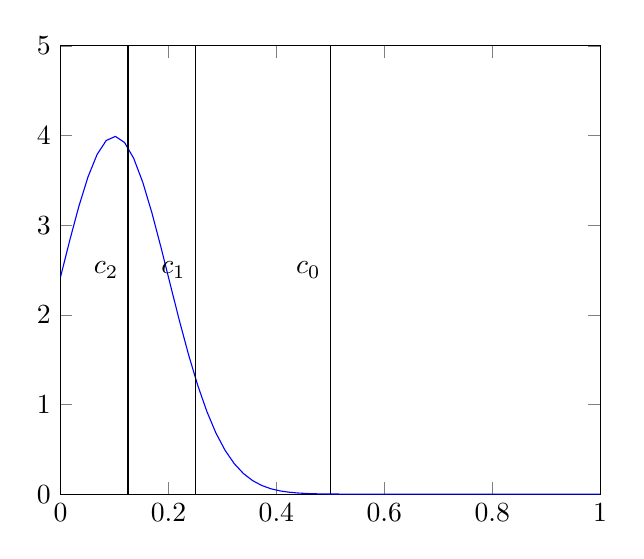
\begin{tikzpicture}
			\def\mean{0.1}
			\def\sigma{0.1}
			\def\pi{3.14159265359}
			\begin{axis}[xmin = 0, xmax = 1, ymin=0, ymax=5, samples=60]
				\addplot[domain = 0:1,blue] {1 / (\sigma * sqrt(2 * \pi)) * exp(-0.5 * ((x - \mean) / \sigma)^2) };
				\draw (axis cs:0.5,0) -- node[left]{$c_0$} (axis cs:0.5,5);
				\draw (axis cs:0.25,0) -- node[left]{$c_1$} (axis cs:0.25,5);
				\draw (axis cs:0.125,0) -- node[left]{$c_2$} (axis cs:0.125,5);
			\end{axis}
		\end{tikzpicture}
	\end{center}
	\caption{3 iterations of binary search with naive initial guess}\label{euclid}
\end{figure}

The underlying distribution is a normal distribution. \TODO{Add reference to section about data}. We can see that the algorithm will have to sweep 3 times over the entire array to get into the region of the actual median. One suggestion for improvement is to use an approximated median as a guess for the first split. We can sample 100 particles and find their median in constant time. Then we will run the binary cut algorithm using the approximated median as an initial guess. This can reduce the runtime by a few iterations, however we cannot make any assessment about the runtime, as this improvement will make the algorithm even slower on some distributions. Let us for example consider the uniform distribution, in this case the addition is pure overhead as the center is already the most accurate initial guess.
\end{comment}



\subsection{Partition Algorithm}\label{sec:part}

We want to continuously update the array storing the positions of the particles and in the words used before, have a direct correlation between $x_i$ and $i$. This enables grouping particles within a cell in a fixed range of two indexes of the particles array. The advantages of this are two fold: Access all particles within a cell in constant time, manipulate particles within a cell using a slice of the array. 

As seen in the pseudo code in figure \ref{proc:part}, the algorithm looks for a pair of particles, where for both the coordinate along the relevant axis are  on the wrong side of the cut plane. In this case the particles can be swapped (line 8) resulting in the correct position of both particles. We refer to \cite{algorithms} for a correctness proof and a more detailed explanation of the algorithm. 

\algnewcommand\And{\textbf{and} }


\begin{figure}[H]
	\begin{algorithmic}[1]
		\Procedure{partition}{$x, cut, axis$}
		\State $i = 0$
		
		\For{$k \in {0,..N - 1}$}
		\If{$\vec{x}_{k, axis} \leq cut$}
		\While{$\vec{x}_{i,axis} \leq cut$ \And $i < N$}
			\State $i = i + 1$
		\EndWhile
		\State $x_{i}, x_{k} = x_{k}, x_{i}$
		\EndIf
		\EndFor
		
		\State $ x_{i}, x_{N_j-1} = x_{N_j-1}, x_{i}$
		\EndProcedure
	\end{algorithmic}
\caption{Partition Method}
\label{proc:part}
\end{figure}

A runtime of $O(N)$ can be derived, as the algorithm iterates over all particles once. Since we need to touch each element at least once to partition the entire array there exists no better method.

Lets apply the algorithm to our running example. We start with our initial array of particles as follows:

\begin{figure}[H]
	\begin{center}
		\csvreader[
		tabular=ccc,
		table head=\hline \bfseries{x} & \bfseries{y} & \bfseries{id} \\\hline,
		late after last line=\\\hline % horizontal line at the end of the table
		]{particles10.csv}{}{\csvcoli & \csvcolii & \csvcoliii}
	\end{center}
\end{figure}

We then partition the particles with a cut in the x axis set to 0.65 as seen in figure \ref{fig:orb2}.

\begin{figure}[H]
	\begin{center}
		\csvreader[
		tabular=ccc,
		table head=\hline \bfseries{x} & \bfseries{y} & \bfseries{id} \\\hline,
		late after last line=\\\hline % horizontal line at the end of the table
		]{particles11.csv}{}{\csvcoli & \csvcolii & \csvcoliii}
	\end{center}
\end{figure}

Finally we partition $cell_2$ into $cell_4$ and $cell_5$ with the cut position 0.55 along the y axis as seen in figure \ref{fig:orb2}. We end up with the following array:

\begin{figure}[H]
	\begin{center}
		\csvreader[
		tabular=ccc,
		table head=\hline \bfseries{x} & \bfseries{y} & \bfseries{id} \\\hline,
		late after last line=\\\hline % horizontal line at the end of the table
		]{particles12.csv}{}{\csvcoli & \csvcolii & \csvcoliii}
	\end{center}
\end{figure}

Note how all particles from $cell_4$ are contained in the range of 0-1. The particles of $cell_5$ in 2-3 and finally the particles contained in the volume of $cell_3$ can be found in 4-7.


\newpage
\section{Theoretical Analysis}

The main goal of this thesis, is to improve the runtime of the ORB algorithm by leveraging the graphics processing unit over the central processing unit. Before implementing, it makes sense to explore if and how strong the performance benefits could in theory manifest itself. For this purpose we develop a simplified model, which we use to compare the CPU version against two different GPU variants. As GPU programming is very low level, the knowledge gained while developing the model also builds a solid theoretical foundation.

\subsection{General Memory Model}\label{sec:gmm}

For a consistent terminology of a computer, we briefly establish a general computing model, which can be applied to most modern high performance systems. We are looking at a single node and its hardware components, a supercomputer may have thousands of these computers linked together where different bandwidth are seen between individual nodes.

Both the CPU and the GPU have their own memory which are connected by a data link, where the the connections are bound by the memory bandwidths. We name the capacity of the CPU memory bandwidth $B_{CPU}$ and the GPU memory bandwidth $B_{GPU}$. There is a separate data link between the CPU and the GPU memory, which is commonly referred to as PCI express or NVLink (for modern NVidia GPU`s, in our model we use the term $I_{GC}$. In systems with multiple CPU there is a link between the individual CPU's which we denote as $I_{CC}$. Finally we call the link between GPUs as $I_{GG}$.

\begin{figure}[H]
	\begin{center}
		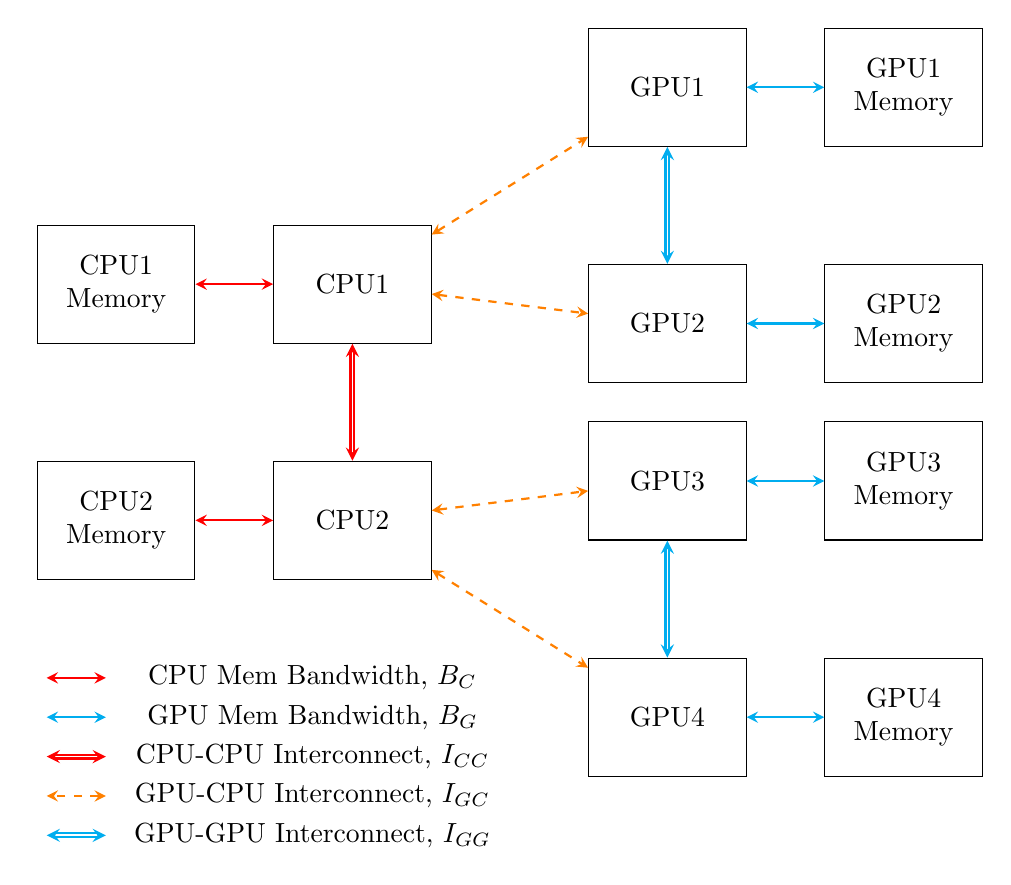
\begin{tikzpicture}
			
			\node[rectangle,
			draw = black,
			text = black,
			anchor = west,
			fill = white,
			align=center,
			minimum width = 2cm, 
			minimum height = 1.5cm] (cpu1) at (0cm,1.5cm) {CPU1};
			
			\node[rectangle,
			draw = black,
			text = black,
			anchor = west,
			fill = white,
			align=center,
			minimum width = 2cm, 
			minimum height = 1.5cm] (cpu2) at (0cm,-1.5cm) {CPU2};
			
			\node[rectangle,
			draw = black,
			text = black,
			anchor = west,
			fill = white,
			align=center,
			minimum width = 2cm, 
			minimum height = 1.5cm] (cpum1) at (-3cm,1.5cm) {CPU1 \\ Memory};
			
			\node[rectangle,
			draw = black,
			text = black,
			anchor = west,
			fill = white,
			align=center,
			minimum width = 2cm, 
			minimum height = 1.5cm] (cpum2) at (-3cm,-1.5cm) {CPU2 \\ Memory};
			
			
			\node[rectangle,
			draw = black,
			text = black,
			anchor = west,
			fill = white,
			align=center,
			minimum width = 2cm, 
			minimum height = 1.5cm] (gpu1) at (4cm,4cm) {GPU1};
			
			\node[rectangle,
			draw = black,
			text = black,
			anchor = west,
			fill = white,
			align=center,
			minimum width = 2cm, 
			minimum height = 1.5cm] (gpu2) at (4cm,1cm) {GPU2};
			
			\node[rectangle,
			draw = black,
			text = black,
			anchor = west,
			fill = white,
			align=center,
			minimum width = 2cm, 
			minimum height = 1.5cm] (gpu3) at (4cm,-1cm) {GPU3};
			
			\node[rectangle,
			draw = black,
			text = black,
			anchor = west,
			fill = white,
			align=center,
			minimum width = 2cm, 
			minimum height = 1.5cm] (gpu4) at (4cm,-4cm) {GPU4};
			
			\node[rectangle,
			draw = black,
			text = black,
			anchor = west,
			fill = white,
			align=center,
			minimum width = 2cm, 
			minimum height = 1.5cm] (gpum1) at (7cm,4cm) {GPU1 \\ Memory};
			
			\node[rectangle,
			draw = black,
			text = black,
			anchor = west,
			fill = white,
			align=center,
			minimum width = 2cm, 
			minimum height = 1.5cm] (gpum2) at (7cm,1cm) {GPU2 \\ Memory};
			
			\node[rectangle,
			draw = black,
			text = black,
			anchor = west,
			fill = white,
			align=center,
			minimum width = 2cm, 
			minimum height = 1.5cm] (gpum3) at (7cm,-1cm) {GPU3 \\ Memory};
			
			\node[rectangle,
			draw = black,
			text = black,
			anchor = west,
			fill = white,
			align=center,
			minimum width = 2cm, 
			minimum height = 1.5cm] (gpum4) at (7cm,-4cm) {GPU4 \\ Memory};
			
			
			\draw[red,  thick, stealth-stealth] (cpum1) to (cpu1);
			\draw[red,  thick, stealth-stealth] (cpum2) to (cpu2);
			\draw[red, double,  thick, stealth-stealth] (cpu1) to (cpu2);
			
			
			\draw[orange, dashed,  thick, stealth-stealth] (cpu1) to (gpu1);
			\draw[orange, dashed,  thick, stealth-stealth] (cpu1) to (gpu2);
			\draw[orange, dashed,  thick, stealth-stealth] (cpu2) to (gpu3);
			\draw[orange, dashed,  thick, stealth-stealth] (cpu2) to (gpu4);
			
			\draw[cyan,  thick, stealth-stealth] (gpum1) to (gpu1);
			\draw[cyan,  thick, stealth-stealth] (gpum2) to (gpu2);
			\draw[cyan,  thick, stealth-stealth] (gpum3) to (gpu3);
			\draw[cyan,  thick, stealth-stealth] (gpum4) to (gpu4);
			
			\draw[cyan, double,  thick, stealth-stealth] (gpu1) to (gpu2);
			\draw[cyan, double,  thick, stealth-stealth] (gpu3) to (gpu4);
			
			
			\node(al) at (-2cm, -3.5cm) {};
			\node (ar) at (-3cm, -3.5cm) {};
			\node[align=left] () at (0.5cm, -3.5cm) {CPU Mem Bandwidth, $B_{C}$};
			\draw[red,  thick, stealth-stealth] (al) to (ar);
			
			\node(al) at (-2cm, -4cm) {};
			\node (ar) at (-3cm, -4cm) {};
			\node[align=left] () at (0.5cm, -4cm) {GPU Mem Bandwidth, $B_{G}$};
			\draw[cyan,  thick, stealth-stealth] (al) to (ar);
			
			\node (bl) at (-2cm, -4.5cm) {};
			\node (br) at (-3cm, -4.5cm) {};
			\node[align=left] () at (0.5cm, -4.5cm) { CPU-CPU Interconnect, $I_{CC}$};
			\draw[red, double,  thick, stealth-stealth] (bl) to (br);
			
			\node (cl) at (-2cm, -5cm) {};
			\node (cr) at (-3cm, -5cm) {};
			\node[align=left] () at (0.5cm, -5cm) { GPU-CPU Interconnect, $I_{GC}$};
			\draw[orange, dashed,  thick, stealth-stealth] (cl) to (cr);
			
			\node (dl) at (-2cm, -5.5cm) {};
			\node (dr) at (-3cm, -5.5cm) {};
			\node[align=left] () at (0.5cm, -5.5cm) { GPU-GPU Interconnect, $I_{GG}$};
			\draw[cyan, double,  thick, stealth-stealth] (dl) to (dr);
			
			
		\end{tikzpicture}
	\end{center}
\end{figure}

\subsection{Datapoints of Supercomputers}

For Piz Daint, Summit and Eiger we have collected all relevant hardware metrics and compiled it into the table seen in figure \ref{fig:datapoints}. Piz Daint and Eiger were chosen, because we have the possibility to test the Code on its systems. Furthermore we include Summit as its is at the time of writing this thesis, one of the most capable supercomputers in the world.

\small
\begin{figure}[H]
	\begin{center}
		\resizebox{\textwidth}{!}{%
		\begin{tabular}{|@{} c | c | c | c | }
			Constant & Piz Daint \cite{piz_daint} & Summit\cite{summit} & Alps (Eiger) \\ 
			\hline
			\# Nodes & 5704 & 4608 & 1024\\
			\# CPUs & 1 & 2 & 2\\
			CPU Model & Intel E5-2690 v3 \cite{E5-2690} & IBM POWER9 & AMD EPYC 7742\cite{AMDEPYC} \\
			CPU Mem. & 64 GB & 256 GB & ?? \\   
			$B_C$  & 68 GB/s & 170 GB/s & 204.8 GB/s x 2	\\
			$I_{CC}$ & - & 64 GB/s & ?? \\
			Base $GHZ_C$ & 2.9 GHZ & 4 GHZ & 2.25 GHZ\\
			Max $GHZ_C$ & 3.8 GHZ & 4 GHZ & 3.4 GHZ\\
			\# Cores & 12 & 22 & 64 \\
			Architexture & Haswell & POWER9 & AMD Infinity Architecture \\
			SIMD & AVX2 & ? & AVX2 \\ 
			\# GPUs & 1 & 6 & 0 \\
			GPU Model & NVIDIA P100 \cite{TESLAP100} & NVIDIA V100s \cite{NVIDIAV100} & - \\
			GPU Mem. Cap. & 16 GB & 16 GB $\times$ 6 & -\\
			$B_G$ & 732 GB/s & 900 GB/s $\times$ 6 & -\\
			$I_{GC}$ & 32 GB/s & 50 GB/s $\times$ 6 & -\\
			$I_{GG}$ & - & 50 GB/s & -\\
			GPU Tflops & 9,3 & 16.5 & -\\
			\# CUDA Cores & 3584 & 5120 & -\\
		\end{tabular}}	
	\end{center}
	\caption{Datapoints of Supercomputers}
	\label{fig:datapoints}
\end{figure}



\subsection{Roofline Performance Model} \label{sec:roof}

In a first step we determine weather our computations are bound by memory bandwidth or the actual performance of the computing unit. The most costly computation is line 6 of the cut method (figure \ref{proc:cut}) with a runtime of $O(32 \times N)$. Oftentimes when an algorithm iterates over a large dataset performing only very little calculations on its individual elements, the limiting factor is the memory. To support this claim make roofline models for all three systems and check weather they are really memory bound. A roofline model compares arithmetic intensity in flops per byte against the actual performance of the computing chip in flops. Therefore we need to gather all the relevant data first.

\subsubsection{Estimating flops}

For modern hardware, its fairly uncommon to release flops (floating point operations per second) values. Steadily evolving SIMD instruction sets result in varying performance for different implementation details, which in turn are compiled into different assembly instructions. Depending on the algorithm, implementation details and compilation flags the c++ compiler tries to compile ideal assembly instruction sets. SIMD instructions can only be used when there is a contiguous memory access, thus in some cases a poor memory layout choice may lead to a much lower flops. 

For most modern CPU chip architectures AVX is the fastest SIMD instruction set available. The common AVX2 enables the processing of 8 floating point operations per instruction with a  CPI (cycles per instructions) of 0.5. The CPI can also vary depending on chip architecture, but to our knowledge all relevant CPU's from figure \ref{fig:datapoints} indeed support a CPI of 0.5 along with AVX2. A lower CPI results in a higher efficiency, as several instructions can be completed in a single cycle. 

We define in equation \ref{eq:avx}, a function to estimate the number of gigaflops for a given hardware. We define GHZ as the gigahertz which can be reached by the CPU, meanwhile $NF$ is the number of floats which can be processed simultaneously using AVX. $CPI$ is as mentioned the cycles per instructions for the AVX instruction set. Finally we have $np$ which is the number of processors, where we assume a perfect parallelization, meaning 100\% of the code can be parallelized.

\begin{center}
	\begin{equation}
		gflops = GHZ * NF * CPI^{-1} * np
	\end{equation}
\label{eq:avx}
\end{center}

Since we have peak flops benchmarks available for the NVIDIA P100 and V100s we do not need to make any estimations on the GPU side.

\subsubsection{Estimating Arithmetic Intensity}

Arithmetic intensity is measured in FLOPS per byte or the number of floating point operations which are computed per byte loaded from memory. The count left part from the cut algorithm (line 6) in figure \ref{proc:cut} can be translated to the following isolated c++ code:

\begin{figure}[H]
	\begin{lstlisting}[language=c++]
		for(auto p= startPtr; p<endPtr; ++p) nLeft += *p < cut;
	\end{lstlisting}
\caption{Counting the particles left of a cut plane}

\end{figure}

Where $p$ is a C-style array which stores the particles position and $nLeft$ stores the number of particles which are smaller than $cut$. We can list the operations per loaded float:

\begin{enumerate}
	\item Compare particle to cut
	\item Add result to $nLeft$
	\item Increment pointer $p$
	\item Compare pointer $p$ with $endPtr$
\end{enumerate}

Which results in a total of 4 operations. Since a single float is stored using 4 bytes, this computes to 1.0 operations per byte or an arithmetic intensity of four. 

Estimating the arithmetic intensity for the GPU is a lot more complicated as it can vary a lot depending on the specific implementation details. But for now we will just assume the same arithmetic intensity as we have had for the CPU.

Note that SIMD instructions do not influence the arithmetic intensity, as the number of floating point operations per byte remains the same. We simply perform a set of operations concurrently. What is however influenced by AVX, is the maximum number of GFLOPS which can be processed by the hardware. If we were to ignore AVX, the algorithm would clearly not be bound by memory, as its performance would lack behind the memory bandwidth. For this reason it is important to consider SIMD instructions.

\subsubsection{The Plots}

Lets us compute the maximally achievable gflops for Piz Daint. To do so, we plug in the corresponding datapoints from figure \ref{fig:datapoints} into the formula \ref{eq:avx} for $np = 1, 2$ and $3$.

\begin{center}
	\begin{equation}
		3.8 * 8 * \frac{1}{0.5} * 2 = 121.6 gflops
	\end{equation}
	\label{eq:daintp1}
\end{center}

\begin{center}
	\begin{equation}
		3.8 * 8 * \frac{1}{0.5} * 4 = 243.2 gflops
	\end{equation}
	\label{eq:daintp2}
\end{center}

\begin{center}
	\begin{equation}
		3.8 * 8 * \frac{1}{0.5} * 8 = 486.4 gflops
	\end{equation}
	\label{eq:daintp3}
\end{center}

The results are depicted as horizontal lines in \ref{fig:roofdaint}. The memory bandwidth is plotted as a line with an equivalent slope. Finally we add a dotted line representing the arithmetic intensity of the Count Left procedure. 
To interpret the roofline mode, one has to follow the dotted line starting from the bottom. Weather it intersect with line representing the maximal performance or the memory bandwidth first, gives an indication weather the program is performance or memory bound. 

\begin{figure}[H]
	\begin{center}
		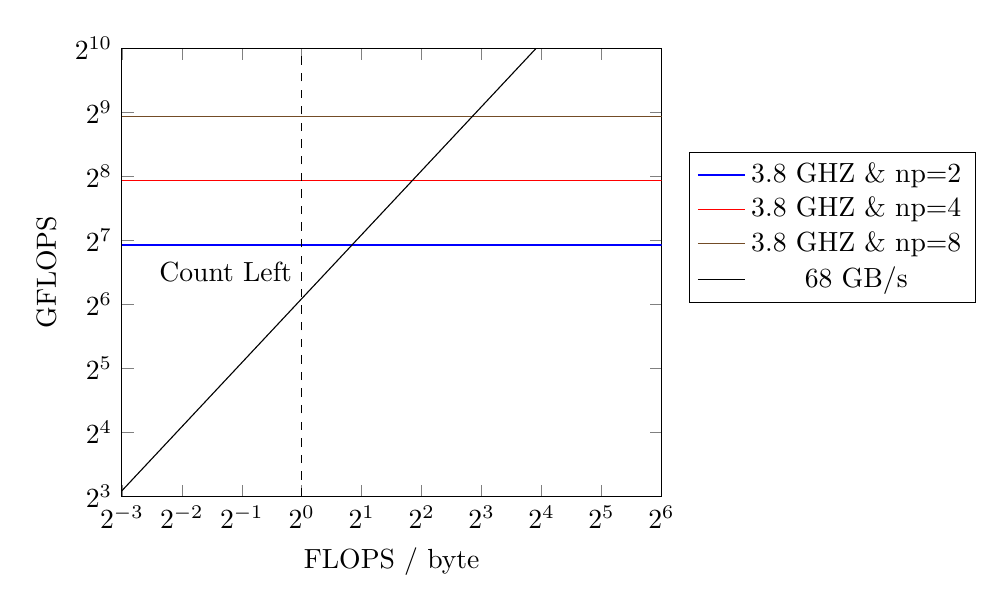
\begin{tikzpicture}
				\begin{axis}[
					xmode=log,
					ymode=log,
					log basis x={2},
					log basis y={2},
					xlabel={FLOPS / byte},
					ylabel={GFLOPS},
					%x filter/.code=\pgfmathparse{#1 + 6.90775527898214},
					xmin = 0.125, xmax = 64, ymin= 8, ymax=1024,
					legend style={at={(1.05,0.6)},anchor=west}]
			
					\addplot+[name path = A, domain = 0.125:64, mark=none] {
						3.8 * 8 * 2 * 2
					};	
					
					\addlegendentryexpanded{3.8 GHZ \& np=2};
					
					\addplot+[name path = A, domain = 0.125:64, mark=none] {
						3.8 * 8 * 2 * 4
					};	
					
					\addlegendentryexpanded{3.8 GHZ \& np=4};
					
					\addplot+[name path = A, domain = 0.125:64, mark=none] {
						3.8 * 8 * 2 * 8
					};	
					
					\addlegendentryexpanded{3.8 GHZ \& np=8};
					
					\addplot+[name path = A, domain = 0.125:64, mark=none] {
						68 * \x
					};	
					
					\addlegendentryexpanded{68 GB/s};
					
		
					\draw[dashed] (axis cs:1,8) -- node[left]{Count Left} (axis cs:1,1024);
					
				\end{axis}
			\end{tikzpicture}
	\caption{Roofline Model for Piz Daint CPU}
	\label{fig:roofdaint}
	\end{center}
\end{figure}


\begin{figure}[H]
	\begin{center}
		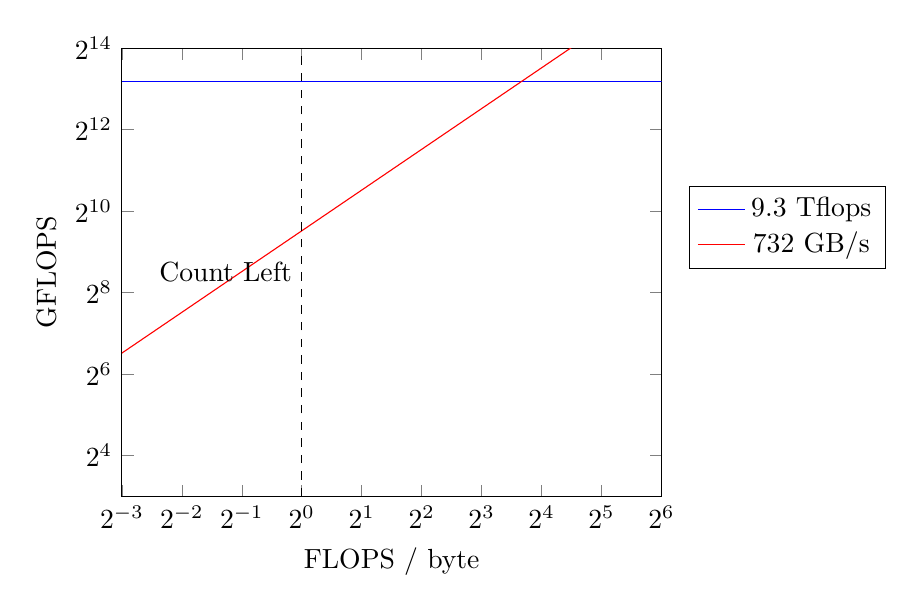
\begin{tikzpicture}
			\begin{axis}[
				xmode=log,
				ymode=log,
				log basis x={2},
				log basis y={2},
				xlabel={FLOPS / byte},
				ylabel={GFLOPS},
				%x filter/.code=\pgfmathparse{#1 + 6.90775527898214},
				xmin = 0.125, xmax = 64, ymin= 8, ymax=16384,
				legend style={at={(1.05,0.6)},anchor=west}]
				
				\addplot+[name path = A, domain = 0.125:64, mark=none] {
					9300
				};	
				
				\addlegendentryexpanded{9.3 Tflops};
				
				\addplot+[name path = A, domain = 0.125:64, mark=none] {
					732 * \x
				};	
				
				\addlegendentryexpanded{732 GB/s};
				
				
				\draw[dashed] (axis cs:1,8) -- node[left]{Count Left} (axis cs:1,16384);
				
			\end{axis}
		\end{tikzpicture}
		\caption{Roofline Model for Piz Daint GPU}
		\label{fig:roofdaintGPU}
	\end{center}
\end{figure}

As it can be seen in figure \ref{fig:roofdaint} and \ref{fig:roofdaintGPU} both the GPU and CPU version running on Piz Daint are memory bound, but due to its much higher memory bandwidth limit, a GPU version should be favored. 

\begin{figure}[H]
	\begin{center}
		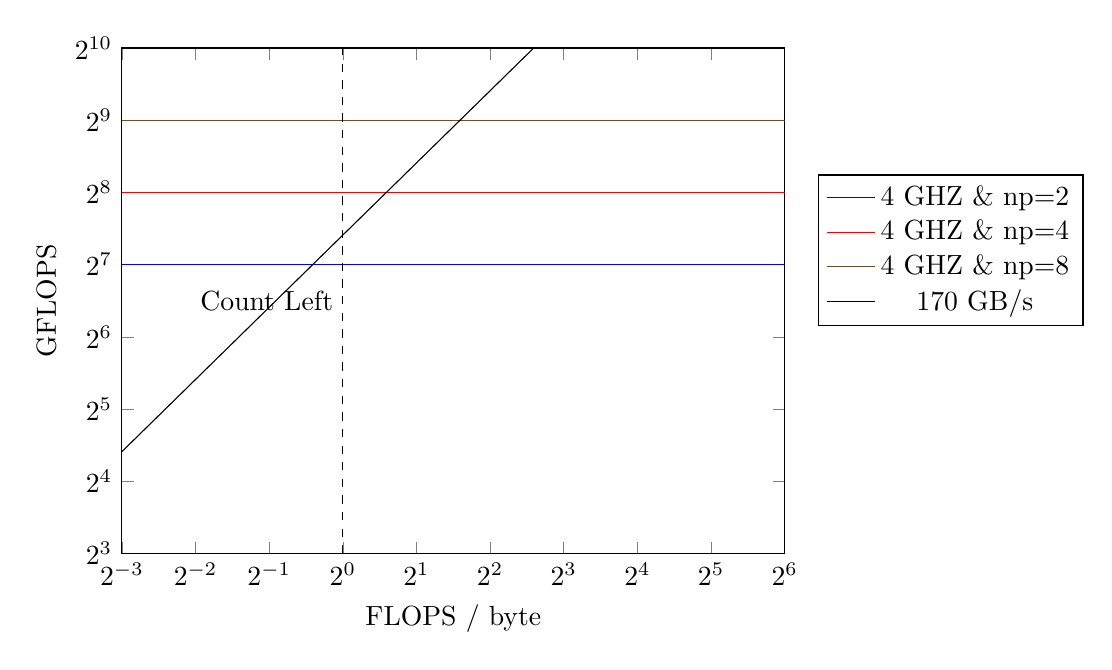
\begin{tikzpicture}
			\begin{axis}[
				xmode=log,
				ymode=log,
				log basis x={2},
				log basis y={2},
				height=8cm,width=10cm, 
				xlabel={FLOPS / byte},
				ylabel={GFLOPS},
				%x filter/.code=\pgfmathparse{#1 + 6.90775527898214},
				xmin = 0.125, xmax = 64, ymin= 8, ymax=1024,
				legend style={at={(1.05,0.6)},anchor=west}]
				
				
				\addplot+[name path = A, domain = 0.125:64, mark=none] {
					4 * 8 * 2 * 2
				};	
				
				\addlegendentryexpanded{4 GHZ \& np=2};
				
				\addplot+[name path = A, domain = 0.125:64, mark=none] {
					4 * 8 * 2 * 4
				};	
				
				
				\addlegendentryexpanded{4 GHZ \& np=4};
				
				\addplot+[name path = A, domain = 0.125:64, mark=none] {
					4 * 8 * 2 * 8
				};	
				
				
				\addlegendentryexpanded{4 GHZ \& np=8};
				
				\addplot+[name path = A, domain = 0.125:64, mark=none] {
					170 * \x
				};	
				
				\addlegendentryexpanded{170 GB/s};
				
				
				\draw[dashed] (axis cs:1,8) -- node[left]{Count Left} (axis cs:1,1024);
			
				
			\end{axis}
		\end{tikzpicture}
	\end{center}
	\caption{Roofline Model for Summit}
	\label{fig:roofsummit}
\end{figure}


\begin{figure}[H]
	\begin{center}
		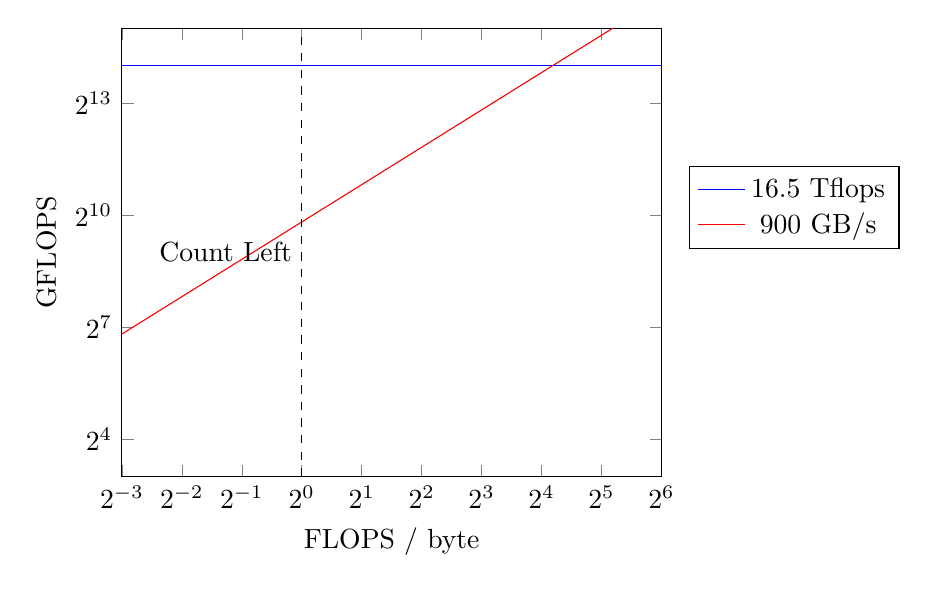
\begin{tikzpicture}
			\begin{axis}[
				xmode=log,
				ymode=log,
				log basis x={2},
				log basis y={2},
				xlabel={FLOPS / byte},
				ylabel={GFLOPS},
				%x filter/.code=\pgfmathparse{#1 + 6.90775527898214},
				xmin = 0.125, xmax = 64, ymin= 8, ymax=32768,
				legend style={at={(1.05,0.6)},anchor=west}]
				
				\addplot+[name path = A, domain = 0.125:64, mark=none] {
					16500
				};	
				
				\addlegendentryexpanded{16.5 Tflops};
				
				\addplot+[name path = A, domain = 0.125:64, mark=none] {
					900 * \x
				};	
				
				\addlegendentryexpanded{900 GB/s};
				
				
				\draw[dashed] (axis cs:1,8) -- node[left]{Count Left} (axis cs:1,32768);
				
			\end{axis}
		\end{tikzpicture}
		\caption{Roofline Model for Summit GPU}
		\label{fig:roofsummitGPU}
	\end{center}
\end{figure}

As visible in figure \ref{fig:roofsummit} and \ref{fig:roofsummitGPU} the same applies to Summit. Its notable how the memory bandwidth only becomes the limiting factor when assuming a parallelization with 4 processors.

\begin{figure}
	[H]
	\begin{center}
		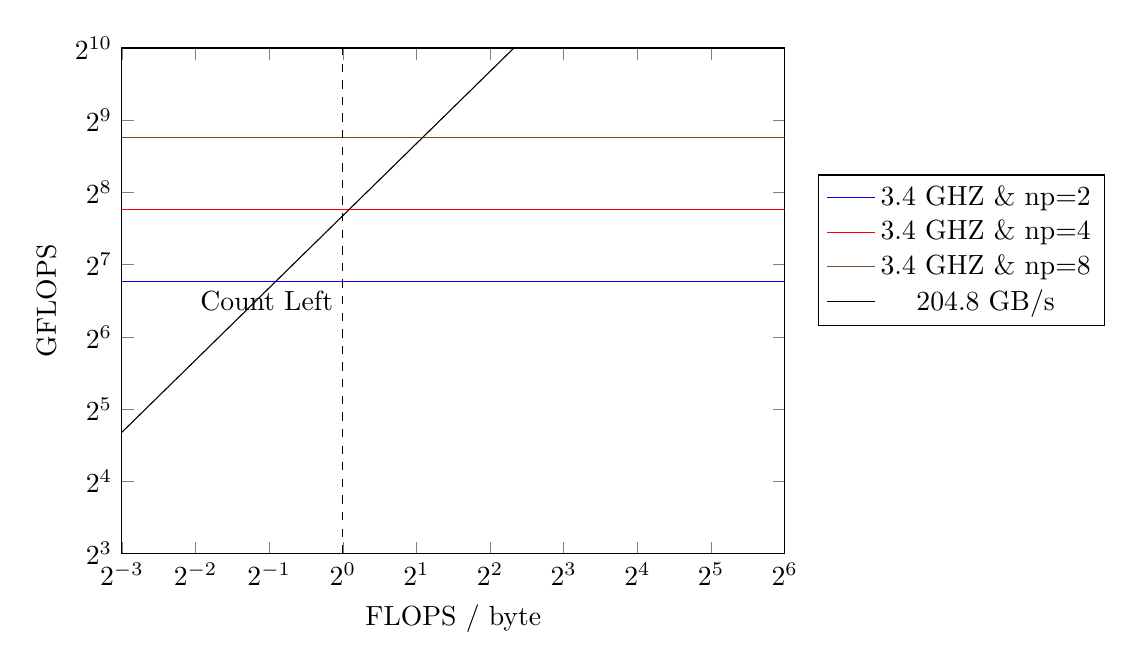
\begin{tikzpicture}
			\begin{axis}[
				xmode=log,
				ymode=log,
				log basis x={2},
				log basis y={2},
				height=8cm,width=10cm, 
				xlabel={FLOPS / byte},
				ylabel={GFLOPS},
				%x filter/.code=\pgfmathparse{#1 + 6.90775527898214},
				xmin = 0.125, xmax = 64, ymin= 8, ymax=1024,
				legend style={at={(1.05,0.6)},anchor=west}]
				
				
				\addplot+[name path = A, domain = 0.125:64, mark=none] {
					3.4 * 8 * 2 * 2
				};	
				
				\addlegendentryexpanded{3.4 GHZ \& np=2};
				
				\addplot+[name path = A, domain = 0.125:64, mark=none] {
					3.4 * 8 * 2 * 4
				};	
				
				\addlegendentryexpanded{3.4 GHZ \& np=4};
				
				\addplot+[name path = A, domain = 0.125:64, mark=none] {
					3.4 * 8 * 2 * 8
				};	
				
				\addlegendentryexpanded{3.4 GHZ \& np=8};
				
				\addplot+[name path = A, domain = 0.125:64, mark=none] {
					204.8 * \x
				};	
				
				\addlegendentryexpanded{204.8 GB/s};
				
				\draw[dashed] (axis cs:1,8) -- node[left]{Count Left} (axis cs:1,1024);
				
				
			\end{axis}
		\end{tikzpicture}
	\end{center}
	\caption{Roofline Model for Alps}
	\label{fig:roofalps}
\end{figure}

Finally alps, which has the highest memory bandwidth compared to its flops, also becomes limited by the bandwidth after using more than four processors.

\subsubsection{Empirical Verification}

We consider a minimal C++ code verify the theoretical model. We use the -S flag along with the g++ compiler to generate assembly code from the c++ source code and make sure that AVX commands are enabled. For testing purposes all entries in the array are set to random values between 0 and 1, and cut is set to 0.5.

In a first test, we do not enable AVX, but turn on $O3$. The generated assembly code looks as follows:

\begin{figure}[H]
	\begin{lstlisting}
.L18:
	movups	(%rax), %xmm0
	addq	$16, %rax
	cmpltps	%xmm2, %xmm0
	psubd	%xmm0, %xmm1
	cmpq	%rdx, %rax
	jne	.L18

	\end{lstlisting}
\caption{Reduction Assembler Code without AVX}
\label{fig:assembler}
\end{figure}
$psubd$ is a packaged instruction, meaning it already uses some form of SIMD instructions. The command is used in the MME and later the SSE2 instruction set. Since we can observe that the $xmm$ registers are used, we know its a SSE2 instruction. 

If we additionally set the compile flag -march=native we end up with the following code:

\begin{figure}[H]
\begin{lstlisting}
.L19:
	vmovups	(%rax), %ymm3
	addq	$32, %rax
	vcmpltps	%ymm2, %ymm3, %ymm0
	vpsubd	%ymm0, %ymm1, %ymm1
	cmpq	%rdx, %rax
	jne	.L19	

\end{lstlisting}
\caption{Reduction Assembler Code with AVX2}
\label{fig:assembler-avx}
\end{figure}

We can identify $vmovups$, $vcomplpts$ and $vpsubd$ which are AVX commands. Since they are using the ymm instead of the xmm registers, we know these are AVX2 and not AVX commands.

\TODO{Fix, Redo this part}
The following test results were achieved from a Intel(R) Core(TM) i9-10885H CPU @ 2.40GHz
processor. We perform the conditional reduction on  $2^{27}$ particles. The reduction takes 244420 microseconds. This means we have a throughput of $2^{27} / 10^{12} * 10^6 / 24420 = 0.00549 tflops$. This of course does not lie anywhere near the theoretical maximum, which even for a single processor ($np = 1$) is $2.4 * 8 * 2 * 1 / 1000 = 0.0384 tflops.$. This is a strong indication, that already with a single processor solutions, we are in the realm of bandwidth limited algorithms. This effect of course, would become even stronger when including parallelism.

But regardless if the app is actually memory bound or not, fact is that the GPU outperforms the CPU by a factor of 10-20 $\times$, thus even if it were bound by the chip architecture, there is still an improvement to be expected when porting the code to the GPU. 

\subsection{Runtime Estimates}

We will construct and explore models for three different approaches. In the first naive implementation, we simply send an array of particles to the GPU, where the counting is then performed. In a more advanced variant, we consider sending the particles from the CPU to GPU only once and perform the partitioning on the GPU as well.  

In order to estimate the runtime of the algorithms we denote the number of particles as $N$. Furthermore we assume a precision $p$ of 32, which is general standard for both integers and floats and its a sensible assumption for astrophysical simulations. We only look at at the positional data of the particles for the runtime analysis since its the only relevant data to be considered to find a cut. The total storage of all particles is $32 \times 3 \times N bits = 4 \times 3 \times N Bytes = 12 \times N Bytes$. Furthermore we assume $d = 1024$ and $N=10^9$.
 
\subsubsection{GPU Counting}

Each time we split all leaf cells into two child cells, we end up with twice the amount of cells. Considering we want to end up with $d$ leaf cells in the end, we need to perform the cut algorithm $log(d)$ times, which corresponds to the height of the tree. Each time we perform the cut algorithm, we test a maximum of $p$ different cut guesses. As we traverse the tree the number of cells increases, but at the same time the number of particles which need to counted decrease by the same factor. Thus the amount of cells which are to be iterated cancels out and we end up with the size of all particles $s$ divide by the memory bandwidth $B_C$.  
 
\begin{center}
	\begin{equation}
			log(d) \times \left ( p \times \frac{ s }{B_{C}} \right ) = t
			\label{eq:cpu}
	\end{equation}
\end{center}

\vspace{5mm}


The Equation \ref{eq:gpu} for the GPU is similar, the only difference being that we use the GPU memory bandwidth $B_{GPU}$ instead of the CPU bandwidth. Furthermore we have to consider the time it takes to send the data from the CPU to the GPU. This adds the terms size divided by CPU to GPU memory bandwidth denoted as $I_{GC}$. Finally we also need to load the data from the CPU memory to the CPU before we are able to send it. 

\begin{center}
	\begin{equation}
			log(d) \times \left ( p \times \frac{s}{B_{G}} + \frac{s}{I_{GC}}  + \frac{s}{B_{C}} \right ) = t
		\label{eq:gpu}
	\end{equation}
\end{center}

\vspace{5mm}


\subsubsection{GPU Counting and Partitioning}\label{gpu-tree-building}

We can also consider performing the partitioning on the GPU, this means that there is no need to send data from the CPU to GPU each time we want to find a cut, allowing us to reduce the costly overheads. This means that we are able to move the considering the CPU GPU bandwidths and the initial loading data out of the bracket and reducing the runtime.

\begin{center}
	\begin{equation}
		log(d) \times \left ( p \times \frac{s}{B_{G}} \right ) + \frac{s}{I_{GC}} + \frac{s}{B_{C}} = t
		\label{eq:gputree}
	\end{equation}
\end{center}


\begin{comment}
\subsubsection{Batch loading}

Finally we can also try to mitigate the overheads introduced by CPU to GPU communication by sending small batches, such that the GPU can already start processing the data, before the data transfer was completed. Lets denote the number of batches by $b$. For the sake of simplicity we only make a single cut and thus can reuse Equation \ref{eq:cpu} for the CPU version. For the GPU we now omit the term for memory access from the GPU. Because we can already start processing data in parallel when the first batch arrived and $B_{G} > I_{GC}$ holds for every modern hardware. Thus the only overhead we still get is $\frac{s \div b}{B_{G}}$ for the very last batch, but as we can just increase b in relation to N, this becomes negligible. Note that this only counts for the very first iteration, thus the only difference we have is the constant of 31 and not 32. 

\begin{center}
	\begin{equation}
		(d-1) \times p \times \frac{s}{B_{G}} + 2 \times \frac{s}{I_{GC}} = t
		\label{eq:gpubatch}
	\end{equation}
\end{center}

Due to possible overhead and no real improvement over the naive GPU version, we will omit the analysis using this method.

\subsubsection{Data compression}

Since for most computer the Interconnect bandwidth is greatly smaller than the Memory bandwidth, we could potentially also think about compressing the particle data. This would increase computational costs, but would allow us to store a higher amount of particles and reduce the cost which comes from loading the particles from memory as well as sending the data over the Interconnect.

\begin{itemize}
	\item Why do we even use floats in the first place? wouldn't integers suit better since precision is uniformly equal?
	\item Reduce transferred number of bits, sacrifice precision?
\end{itemize}

\TODO{Add plots?}

\end{comment}
\newcommand\s{12}

\newcommand\p{32}

%\newcommand\d{1024}

\normalfont
\subsection{Piz Daint} 

Let us plugin the values from figure \ref{fig:datapoints} into the corresponding formulas \ref{eq:cpu}, \ref{eq:gpu} and \ref{eq:gputree} for piz daint.

\subsubsection{Naive implementation}
The naive implementation yields the following speeds for the naive CPU  implementation:

\pgfmathsetmacro\cpuPiz{ln(1024) / ln(2) * (\p * \s / 68)}

\begin{center}
	\begin{equation}
		log(1024) \times \left ( \p \times \frac{ \s GB }{68 GB/s} \right )  = \cpuPiz s
	\end{equation}
\end{center}


And the corresponding GPU implementation:
\pgfmathsetmacro\gpuPizN{ ln(1024) / ln(2) * (\p * \s / 732 + \s / 32 + \s / 68)}
\begin{center}
	\begin{equation}
		log(1024) \times \left ( 32 \times \frac{12 GB}{732 GB/s} + \frac{12 GB}{32 GB/s}  + \frac{12 GB}{68 GB/s} \right )=  \gpuPizN s
	\end{equation}
\end{center}

This yields in a speed-up of:
\pgfmathsetmacro\speedup{\cpuPiz / \gpuPizN}
\begin{center}
	\begin{equation}
		\frac{\cpuPiz}{\gpuPizN} = \speedup \times
	\end{equation}
\end{center}


\subsubsection{GPU Tree Building}

And the corresponding GPU implementation:
\pgfmathsetmacro\gpuPizT{ ln(1024)/ln(2) * (\p * \s / 732)  + \s / 32 + \s / 68}
And the corresponding GPU implementation:
\begin{center}
	\begin{equation}
		log(1024) \times \left ( \p \times \frac{\s GB}{732 GB/s} \right ) + \times \frac{\s GB}{32 GB/s}  + \frac{\s GB}{68 GB/s} = \gpuPizT s
	\end{equation}
\end{center}

This yields in a speed-up of:
\pgfmathsetmacro\speedup{\cpuPiz / \gpuPizT}
\begin{center}
	\begin{equation}
		\frac{\cpuPiz}{\gpuPizT} = \speedup \times
	\end{equation}
\end{center}

\vspace{5mm}

\pgfmathsetmacro\cpuSummit{ln(1024) / ln(2) * (\p * \s / (170 * 2)}
\pgfmathsetmacro\gpuSummitN{ln(1024) / ln(2) * (
	(\p * \s / (900 * 6) + 
	\s / (50 * 6) + \s /(170 * 2)
	)}
\pgfmathsetmacro\gpuSummitT{ln(1024) / ln(2) * 
	(\p * \s / (900 * 6))
	+  \s / (50 * 6) + \s /(170 * 2)}
\pgfmathsetmacro\cpuEiger{ln(1024) / ln(2) * (\p * \s / (204.8 * 2)}
 
The computations for Eiger and Summit can performed in the same way as we have shown for Piz Daint. For Eiger we cannot make any assumption for a GPU version as its CPU only system.

\begin{comment}

\subsection{Summit}

Let us plugin the values from Figure \ref{fig:datapoints} into the corresponding formulas \ref{eq:cpu}, \ref{eq:gpu}, \ref{eq:cputree} and \ref{eq:gputree}.

\subsubsection{Naive implementation}
The naive implementation yields the following speeds for the naive CPU  implementation:


\begin{center}
	\begin{equation}
		log(1024) \times \left ( \p \times \frac{ \s GB }{170 GB/s \times 2} \right ) = \cpuSummit s
	\end{equation}
\end{center}

And the corresponding GPU implementation:

\begin{center}
	\begin{equation}
		log(1024) \times \left ( \p \times \frac{\s GB}{900 GB/s \times 6} + \frac{\s GB}{50 GB/s \times 6}  + \frac{\s GB}{170 GB/s \ \times 2} \right )= \gpuSummitN s
	\end{equation}
\end{center}

This yields in a speed-up of:
\pgfmathsetmacro\speedup{\cpuSummit / \gpuSummitN}
\begin{center}
	\begin{equation}
		\frac{\cpuSummit s}{\gpuSummitN s} = \speedup \times 
	\end{equation}
\end{center}


\subsubsection{GPU Tree Building}

And the corresponding GPU implementation:

\begin{center}
	\begin{equation}
		log(1024) \times \left ( \p \times \frac{\s GB}{900 GB/s \times 6} \right ) + \frac{\s GB}{50 GB/s \times 2}  + \frac{\s GB}{170 GB/s \times 2} = \gpuSummitT s
	\end{equation}
\end{center}

This yields in a speed-up of:
\pgfmathsetmacro\speedup{\cpuSummit / \gpuSummitT}
\begin{center}
	\begin{equation}
		\frac{\cpuSummit s}{\gpuSummitT s} = \speedup \times
	\end{equation}
\end{center}


\vspace{5mm}


\subsection{Eiger}

\pgfmathsetmacro\cpuEiger{ln(1024) / ln(2) * (\p * \s / (204.8 * 2)}

\begin{center}
	\begin{equation}
		\log(1024) \times \p \times \frac{ \s GB }{204.8 GB/s \times 2} = \cpuEiger s
	\end{equation}
\end{center}

\end{comment}

\subsection{Conclusion}

We conclude that the GPU version with GPU Tree building enabled yields the best speedup and also performs a lot better than the CPU version. Furthermore we can observe that the speedup is bounded by $\frac{B_{GPU}}{B_{CPU}}$/, because both the CPU and GPU implemented version are ultimately limited by the bandwidth.

\begin{figure}[H]
	\begin{center}
		\begin{tikzpicture}
			
			\begin{axis} [ybar,height=10cm,width=13cm, 
				bar width=0.8cm,
				enlargelimits=0.2,
				symbolic x coords={Piz, Summit, Eiger},
				legend columns=1,
				legend entries={CPU, Hybrid Naive, Hybrid Tree},
				ylabel={Runtime (s) },
				x tick label style={rotate=45,anchor=east}, 
				xtick=data]
				\addplot coordinates {
					(Piz,\cpuPiz ) 
					(Summit,\cpuSummit) 
					(Eiger,\cpuEiger) 
				};
			
				\addplot coordinates {
					(Piz,\gpuPizN ) 
					(Summit,\gpuSummitN ) 
				};
			
				\addplot coordinates {
					(Piz,\gpuPizT ) 
					(Summit,\gpuSummitT  ) 
				};
			\end{axis}
			
		\end{tikzpicture}
	\end{center}

\caption{Execution times of different strategies}
\label{fig:exectimes}
\end{figure}




\begin{comment}
\begin{figure}
\begin{center}
\begin{tikzpicture}
\begin{axis}[xmin = -1, xmax = 13, ymin=-1, ymax=6]
\addplot[domain = 0:12,blue] {ln(1024) / ln(2) * 
(\p * x / (900 * 6))
+  x / (50 * 6) + x /(170 * 2)};
\addplot[domain = 0:12,blue] {ln(1024 * 16) / ln(2) * 
(\p * x / (900 * 6))
+  x / (50 * 6) + x /(170 * 2)};
\end{axis}
\end{tikzpicture}
\end{center}
\caption{??}
\label{fig:exectimes}
\end{figure}

\end{comment}

\newpage
\section{CPU Implementation}

In this section describe the stand-alone implementation of the accelerated ORB algorithm using CPU acceleration only. Building on the CPU version, we introduce possible improvements to selected parts of the code in the next section \ref{sec:gpuimpl}. 

We develop somewhat separately from the PKDGrav codebase in order to keep the project smaller and more easily understandable. However we make use of mdl from PKDGrav, which can be used to distribute the workload among nodes and processors on a single chip. This reduces the complexity and we do not have to worry about communication methods and CPU parallelism too much. Since the parallelization are abstracted using mdl, we only use the term threads when referring to computation units. Individual threads might be computed on a different node, or on a different processor on the same node, but this does not change things from an implementation side.

We refrain from describing each part of the code in detail, however any performance critical details and all the important data-structures are described. Furthermore, we will pay special attention to the CUDA kernels and also memory management strategies for several reasons: minor implementation details can have a big impact upon the performance and increased replicability of the results.

A brief overview of the core elements are:

\begin{itemize}
	\item \textbf{particles}: The particles array has ownership over all particle objects. It has the shape of a multidimensional array, where the first three axes are occupied by positional data and the rest can be filled with meta data.
	\item \textbf{Cell}: The cell class is a structure keeping track of the fundamental cell information. In essence it is the analogue to the concept of the $cell$ which we have already introduced in section \ref{section:orb}.
	\item \textbf{Services}: The services are a set of functions, which together form the building block of the ORB algorithm. This abstraction layer allows us to dynamically distribute and collect tasks from different processors. Each service builds on top of a PST class which is introduced by mdl2.
	
\end{itemize}

For this project we will use C++ 17 along with CUDA 11.3, OpenMPI 4.1.0 and Blitz++ 1.0.2 \cite{blitzcpp}. 

\subsection{MDL}

MDL is essentially an abstraction layer around a multiprocessor communication as well as a multiprocessor scheduler. It decomposes threads into worker and a master threads and builds a tree hierarchy around the threads. The coordination works with a object called services, where the master can start services, the service objects then traverse the tree of threads until every thread has received the input data of the service. A service can be run via a method called $RunService$ where the input data is given via simple pointers. With the help of void pointers, we can use any object or array of objects as an input or output of the service. 

\subsection{Particles}

We use C-style arrays interchangeably with blitz++ arrays to store all particles. blitz++ is a wrapper class around C-style arrays, which helps with pointer management and can speed up the debugging process by keeping track of the array boundaries. Furthermore it features array slicing and does its own memory management. In certain cases we need to access the actual C-style array, which can be accessed with $array.data()$, for example iterating over the Blitz++ array is observed to compile to optimized assembly instructions which do not leverage the latest SIMD instructions as explained in section \ref{sec:roof}.

The array has a (N,3) shape where each row represents a single particle. To enable coalesced memory access when iterating over a single axis i.e. $x_{:, axis}$, we choose a row major storage order, over a column major storage order. Even though column accesses patterns i.e. $x_{i,:}$ are used as well, they happen less frequently. Most importantly there are cases where entire section of a row have to copied, which is by magnitude faster with row major storage.


\subsection{Cell}

Quickly building and accessing elements of the SPTDS generated by ORB requires a suitable data structure. Instead of a tree with pointers, we can use a heap since the necessary conditions for a nearly complete binary tree are met as seen in section \ref{section:orb-example}. Elements within a heap can be accessed and added in constant runtime. Depicted in figure \ref{fig:treeheap} is the finished SPTDS of the sample dataset stored as a heap.

\begin{figure}[H]
	\begin{center}
		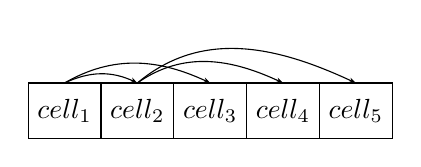
\begin{tikzpicture}[
			%  -{Stealth[length = 2.5pt]},
			start chain = going right,
			node distance = 0pt,
			MyStyle/.style={draw, minimum width=2em, minimum height=2em, 
				outer sep=0pt, on chain},
			]
			\node [MyStyle] (1) {$cell_1$};
			\node [MyStyle] (2) {$cell_2$};
			\node [MyStyle] (3) {$cell_3$};
			\node [MyStyle] (4) {$cell_4$};
			\node [MyStyle] (5) {$cell_5$};
			\begin{scope}[-{Stealth[length = 2.5pt]}]
				\draw (1.north) [out=25, in=155] to (2.north);
				\draw (1.north) [out=30, in=155] to (3.north);
				\draw (2.north) [out=35, in=155] to (4.north);
				\draw (2.north) [out=40, in=155] to (5.north);
			\end{scope}
		\end{tikzpicture}
		\qquad
		\begin{figure}
			\Tree[.cell_1 [.cell_2 [.cell_4 ] [.cell_5 ] ]
			[.cell_3 ]]
		\end{figure}
	\end{center}
	\caption{Tree as heap}
	\label{fig:treeheap}
\end{figure}

An array can be used as an efficient storage medium for the heap, since in our case $d$ can be set at compile time and the maximum number of cells in the SPTDS can be derived from that. Meaning the array can be allocated statically.
Because mdl communicates data as arrays between the threads, another advantage of the array storage is the absence of any costly data structure conversion. 

Since the STPDS is only a nearly complete binary tree and not a complete binary tree, we have to be careful when iterating over the levels of three, as the very last level is not filled entirely with cells. But because $d$ is known, many attributes of the SPTDS can determined deterministically.

\subsubsection{Heap Conditions}
As with all heap data-structures we have the following conditions:

\begin{itemize}
	\item The root cell has index 1
	\item The left child of cell at index $i$ can be accessed at the index $i\times2$. 
	\item The left child of cell at index $i$ can be accessed at the index $i\times2 + 1$. 
\end{itemize}

\begin{figure}[H]
	\centering
	\begin{forest}
		[$cell_1$
		[$cell_2$ [$cell_4$] [$cell_5$]][$cell_3$]  
		]
	\end{forest}
	\caption{Tree with $d$ = 3}
	\label{fig:extree}
\end{figure}

\vspace{0.5cm}
We can derive the following constraints given the number of leaf cells $d$. 

\begin{itemize}
	\item We can compute the depth of the tree with: $\lceil log_2(d) \rceil$
	\item The number of leaf cells on the second last level is given by $2^{depth} - d$ 
	\item There are exactly $2 \times d - 2^{depth}$ items (which must all be leaf cells) on the last level. 
	\item The total number of cells are $2\times d - 1$.
\end{itemize}

In the example tree depicted in figure \ref{fig:extree} we indeed observe that the depth corresponds to: $\lceil log_2(d) \rceil = 2$, the number of leaves on the second last level is  $2^{2} - 3 = 1$ and the number of leaves on the last level are $2 \times 3 - 2^{2} = 2$. Finally the total number of cells is $2\times 3 - 1 = 5$.

\subsubsection{Class}
The cell class consists of the following variables:

\begin{itemize}
	\item $id$: Unique identification of the cell instance and corresponds to its index in the heap array plus one. The plus one comes from the different indexing for heap constraints, where we start with 1, and the classic array indexing starting with 0. It can be used to compute  indices of both child cells and parent cells using the above shown formulas.
	\item $nLeafCells$: Equivalent to  $d_{cell}$ and depicts the number of leaf cells to be found in all of its successors. Its used when building the tree, to track weather a cell needs to be split or not. 
	\item $lower$: 3D point coordinate representing the lower boundary corner of the 3D volume $V_{cell}$ which is encompassed by this cells.
	\item $upper$: Represents the upper boundary corner of the volume.	
	\item $cutAxis$: Stores the axis where the cut plane is to be searched for. 
	\TODO{LOD??}
\end{itemize}

\subsection{Mapping cells to particles}

The SPTDS is consistent across all nodes, therefore it is stored on a single thread, also named master thread in mdl. Very often we need to know which particles are encompassed in the volume of which cell and since the particles are distributed among the threads. Thus we introduce a data structure to keep track of the relation between cells and its particles. 
Thanks to the partitioning algorithm all particles belonging to a single cell can be found in a consecutive section of the particles array. Thus we can use a 2D array, where for each cell we store the corresponding range as a tuple, making the size of the array equivalent to the total number of cells $2 \times d -1$ multiplied by two. We name the data structure $cellToRangeMap$ and it is stored in the local data of each pst, meaning each thread has a different version the $cellToRangeMap$ array. Furthermore this implies that the data structure needs to be updated across all threads whenever we perform a partition.


\subsection{Services}


There are several implementation of services, but in our case we make use of the traverse combine service. As the name says, it traverses the tree of threads until all threads are reached, then the predefined computations are executed on the input data. After the computations have finished, the results traverse the tree in the opposite direction, until they reach the master thread which initialized the service in the first place. MDL also exposes a function which allows us to define, how we treat two data packages when they are combined.

The most important services for the CPU version are:


\begin{itemize}
	\item $init$ : Reads the particles and allocates memory on the CPU accordingly.
	\item $finallize$ : Frees all the memory and ensures a memory leak free execution.  
	\item $countLeft$ : Counts the number of particles left of a provided cut position for each of the cells.
	\item $makeAxis$ : 
	\item $count$ : Counts the total number particles inside the domain for each of the provided cells.
	\item $partition$ : Partitions the particles to preserve memory locality.
\end{itemize}




\subsubsection{Count Left}

The countLeftService takes as a input an array of cells and stores the counts in an output array. Each cell comes with a cut position and a cut axis, thus the service counts the number of particles to the left of this position in the given axis. 

As for every service, we have access to the input array with a pointer to its first element in memory called $in$ and correspondingly $out$ for the output array. We then iterate over the number of cells and access the cell structure given the cellPtrOffset as seen on line number two.
We then check weather the proper cut has already been found, if so we directly continue with the next cell (Line 4-6). We use the cellToRangeMap, which is stored as local data of the pst to retrieve the begin and end index of this cell in the particles array. (Line 7-8).
We then take a slice of the particles array and store a pointer to the data in $startPtr$ and correspondingly compute the end pointer as well. (10-14).
Finally we simple iterate over the particles and count up, as previously mentioned, this can enable AVX, given hardware support and the proper compile flags. Usually $-march=native$ along with $O3$ will enable AVX. 

\begin{lstlisting}[language=c++]
	for (int cellPtrOffset=0; cellPtrOffset<nCells; ++cellPtrOffset){
		auto cell = static_cast<Cell>(*(in + cellPtrOffset));
		
		if (cell.foundCut) {
			continue;
		}
		int beginInd = pst->lcl->cellToRangeMap(cell.id, 0);
		int endInd =  pst->lcl->cellToRangeMap(cell.id, 1);
		
		blitz::Array<float,1> particles =
		pst->lcl->particlesAxis(blitz::Range(beginInd, endInd));
		
		float * startPtr = particles.data();
		float * endPtr = startPtr + (endInd - beginInd);
		
		int nLeft = 0;
		float cut = cell.getCut();
		for(auto p= startPtr; p<endPtr; ++p)
		{
			nLeft += *p < cut;
		}
		
		out[cellPtrOffset] = nLeft;
	}
\end{lstlisting}


\subsubsection{Count}

Counting the total number of particles is very trivial, given the cellToRange map. 

\begin{lstlisting}[language=c++]
	for (int cellPtrOffset=0; cellPtrOffset<nCells; ++cellPtrOffset) {
		auto cell = static_cast<Cell>(*(in + cellPtrOffset));
		out[cellPtrOffset] = 
		lcl->cellToRangeMap(cell.id,1) - 
		lcl->cellToRangeMap(cell.id,0);
	}
	
\end{lstlisting}

\subsubsection{Partition}
The local reshuffle service is responsible for rearranging the particles in such a way, that each range in the particles array, corresponds to a single cell. 
Its implementation is equivalent to a hoare partition. The implementation is straight forward and there exists no known way to improve this, at least from an algorithmic perspective. There might be some ways to explore in terms of memory access speed, or even porting the algorithm to CUDA. 

On line 31 till 37 we also update the cellToRangeMap in order to reflect the changes we have made in the particles array.

\begin{figure}[H]
	\begin{lstlisting}[language=c++]
		for (int cellPtrOffset=0; cellPtrOffset<nCells; ++cellPtrOffset){
			auto cell = static_cast<Cell>(*(in + cellPtrOffset));
			
			int beginInd = pst->lcl->cellToRangeMap(cell.id, 0);
			int endInd = pst->lcl->cellToRangeMap(cell.id, 1);
			
			int i = beginInd-1, j = endInd;
			float cut = cell.getCut();
			
			while(true)
			{
				do
				{
					i++;
				} while(lcl->particles(i, cell.cutAxis) < cut && i <= endInd);
				
				do
				{
					j--;
				} while(lcl->particles(j, cell.cutAxis) > cut && j >= beginInd);
				
				if(i >= j) {
					break;
				}
				
				swap(lcl->particles, i, j);
			}
			
			swap(lcl->particles, i, endInd -1);
			
			lcl->cellToRangeMap(cell.getLeftChildId(), 0) =
			lcl->cellToRangeMap(cell.id, 0);
			lcl->cellToRangeMap(cell.getLeftChildId(), 1) = i;
			
			lcl->cellToRangeMap(cell.getRightChildId(), 0) = i;
			lcl->cellToRangeMap(cell.getRightChildId(), 1) =
			lcl->cellToRangeMap(cell.id, 1);
			
		}
	\end{lstlisting}
\end{figure}


\subsubsection{Make Axis}

As mentioned in section \ref{sec:multipole} the relevant axis to search for the cut position differs for each cell. Therefore we cannot simply iterate over a single array, we need to iterate over the relevant axis instead. In order to simplify the process we introduce a service which copies iterates over all cells and copies the slice of coordinates which are encompassed in its volume and lie on its cut axis to a temporary array.



\subsection{Parallel implementation of ORB }\label{sec:parellize-orb}

In the context of parallelization, we define the number of processors as $np$. When the goal of the algorithm is workload balancing, we will want to set $d = np$ to end up with exactly as many leaf cells as we have processors. In the context of a supercomputing system $np$ is usually equivalent to the number of nodes in the system.

Initially we assume that each processor has a random unique subset of all the particles stored in its memory, this has two reasons. For one we run into memory limitations quickly when trying to load all the particles onto a single node, furthermore memory bandwidths limitations can be multiplied by the number of processors and are thus a lot higher. 

Let us now apply this to our running example where we have 3 nodes.

\begin{figure}[H]
	
	\centering
	\begin{tikzpicture}
		\begin{axis}
			[
			nodes near coords,
			xmin=-0.,
			xmax=1.,
			ymin=-0.,
			ymax=1.,
			title=Recursion depth 0,
			legend cell align=left
			]
			
			\addplot    +[
			only marks,
			point meta=explicit symbolic,
			restrict expr to domain={\thisrow{o1}}{0:0}, 
			] table [
			x=x, 
			y=y, 
			meta=id, 
			col sep=comma] 
			{particles10.csv};
			
			\addplot    +[
			only marks,
			point meta=explicit symbolic,
			restrict expr to domain={\thisrow{o1}}{1:1}, 
			] table [
			x=x, 
			y=y, 
			meta=id, 
			col sep=comma] 
			{particles10.csv};
			
			\addplot    +[
			only marks,
			point meta=explicit symbolic,
			restrict expr to domain={\thisrow{o1}}{2:2}, 
			] table [
			x=x, 
			y=y, 
			meta=id, 
			col sep=comma] 
			{particles10.csv};
			
			\legend{$p0$,$p1$,$p3$}
			
			%\draw [fill=red!20](0.0,0.0) rectangle (1, 1);
			%\node[below] at (0.5, 1){$cell_1$};
		\end{axis}
	\end{tikzpicture}
	\caption{Example particles distributed randomly across 3 nodes}
\end{figure}

The ORB algorithm is only executed form the operative node, all other nodes are purely worker nodes and perform certain parts of the algorithm. In our case one of the most performance intensive tasks is found on line 6 from the cut procedure as seen in figure \ref{proc:cut}. Not only is it costly, its also a task that can only be executed from the node, which owns the particles array, i.e. its stored in its memory. Therefore the worker nodes count the number of particles on the left side of a 2D cut plane individually and send back the results to the operative thread as seen in figure \ref{fig:orbp}. Besides the counting we also have the partitioning which also concerns the particles array and thus can only be executed by its corresponding owner. Consequently the procedure is also executed on the worker nodes individually. Note that the operative node can also perform work, thus become a worker node at times. This can be seen in figure \ref{fig:orbp}, where p0 is the operative node, but still performs partition and counting operations.

\begin{figure}[H]
	\begin{center}
		\begin{tikzpicture}
			
			\timeline{6}{13}{3}
			
			
			\parallelloop{-2}{11.5}{8}{1.5}{loop till tree built};
			
			\parallelloop{-1}{9.5}{7}{5.5}{loop till cut found};
			
			\communication{Init}{0}{7}{12};
			
			\communication{Count}{0}{7}{11};
			
			
			\communication{Make Axis}{0}{7}{10};
			
			\communication{Count Left}{0}{7}{9};
			
			\process{improve \\ cut}{0}{8};
		
			
			\communication{Partition}{0}{7}{5};
			
			\communication{Finalize}{0}{7}{1};
			
			\process{generate\\ new \\ cells}{0}{4};
			
		\end{tikzpicture}
	\end{center}
	\caption{Parallelized ORB CPU version}
	\label{fig:orbp}
\end{figure}



\newpage
\section{GPU Implementation}\label{sec:gpuimpl}

CUDA is programming language developed by NVIDIA allowing us to write code which is run directly on the graphics card.

Note that the total number of particles, which can be simulated, will be reduced in both implementations, as the GPU memory is a lot smaller than the CPU memory. One could propose to load and offload several batches from the CPU to GPU but, this comes with a significant overhead due to the slow memory bandwidth between the CPU and the GPU $I_{GC}$.


\subsection{Relevant CUDA Concepts}

CUDA gives us the ability to launch kernels, which are written in C with some additional CUDA specific syntax. These kernel can be run from the CPU, commonly refereed to as the host, and are then executed on the GPU, also known as the device. The device and the host have a separate memory and as seen in section \ref{sec:gmm} the transfer $I_{CG}$ rates between the GPU and CPU are generally slower, under performing $I_{C}$ and $I_G$ speeds. Therefore one of key the challenges when rewriting CPU code to GPU code is to limit data transfers between the GPU and CPU as much as possible. Furthermore we have divide our problems into subproblems, where each subproblem is then executed on a block. CUDA cannot give any guarantees considering the order of execution of these blocks, therefore we have to fundamentally rethink algorithms when porting them from CPU to GPU code, where some algorithms are more or less fitted. Generally we only think about problems which are applied on large data arrays, the less connection between the individual results exists, the easier it is to implement an GPU version of the computation. Furthermore we can assume that problems with less branching work better on the GPU due to various reasons, which we will explain in detail later. 

Building a tree is therefore a rather challenging problem as there are many computations which influence another and building a tree involves a lot of branching, at least when it is done in a conventional manner. 

\begin{figure}[H]
	\begin{lstlisting}[language=c++]
add<<<
	nBlocks,
	nThreads,
	nThreads * bytesPerThread,
	stream
>>>(
	param1,
	param2
);
	\end{lstlisting}
\caption{Calling a CUDA kernel}
\label{cuda:call}
\end{figure}

A kernel is executed exactly once for every kernel, where a block consists of many kernels. The number of kernels per block and the total number of blocks can be defined by the user as seen in the kernel call syntax in figure \ref{cuda:call} on line 2 and 3. 


\subsubsection{Warps}

Each consecutive grouping of 32 threads form a warp. All threads within a warp are executed in parallel, given that there is no warp divergence. Because warps are executed in parallel, there is no need for synchronization between the threads of the same warp. A warp divergence can occur, if there is a control statements, where two or more threads from the same warp execute a different code. This leads to a decrease in performance and should be avoided whenever possible.

\subsubsection{Memory}

Each block has access to shared memory register, where the capacity of this register can be defined at runtime by the host as seen in figure \ref{cuda:call} on line 4. The maximum shared memory size depends on the hardware but usually there are 48kB per block available. There are also upper limits for the number of threads per block, usually \TODO{B or b??} around 512 to 1024. With a shared memory size of 48kb and 1024 threads we get $\frac{48000b}{1024} = 46b$ per thread. This is equivalent to a little bit more than one float per thread. However usually we do not max out the thread counts per block, leaving us with more shared memory space per thread. 

Data in the shared memory exists only as long as the kernel exists and it cannot be accessed across different blocks. Race conditions do apply to shared memory, but threads in a block can be synchronized, therefore it is not safe to have writes from multiple threads on the same shared memory address. There exists a CUDA command $\_\_synchtreads()$ which allows us to synchronize all threads within a block, enabling us to control the execution order of individual statements.

Additionally to the shared memory, there exists global memory. Global memory is persistent even after a block or a kernel has finished and is the only way to send data between the device and the host. Since the data is not deleted after a kernel has finished, we can and should reuse the data whenever possible for other kernels, reducing the memory transfer overhead. Global memory is significantly slower than shared memory and it is best practice to copy data from global memory to shared memory before performing actual computations on it, thus reducing the total number of memory accesses on global memory. After the computations have finished, the results can be written back from shared to global memory.

\subsubsection{Memory Access Patterns}

Global memory is fetched from memory in 32 Byte packages, which translates to $\frac{32}{4} = 8$ floats. A simple aligned sequential memory access pattern, where each tread reads a single float from global memory, results in 4 transaction per warp (32 threads). Unaligned memory access can have minor performance penalties because more memory banks have to be loaded per warp. 

For shared memory each bank consists of 32 bits, which translates to a 32 bit precision number. If 32 unique threads access 32 different banks, then its considered an ideal access pattern, because the banks can be loaded in parallel. If however multiple threads access the same memory, a bank conflict is introduced and the access speed is greatly reduced.




\begin{figure}[H]
	\begin{center}
		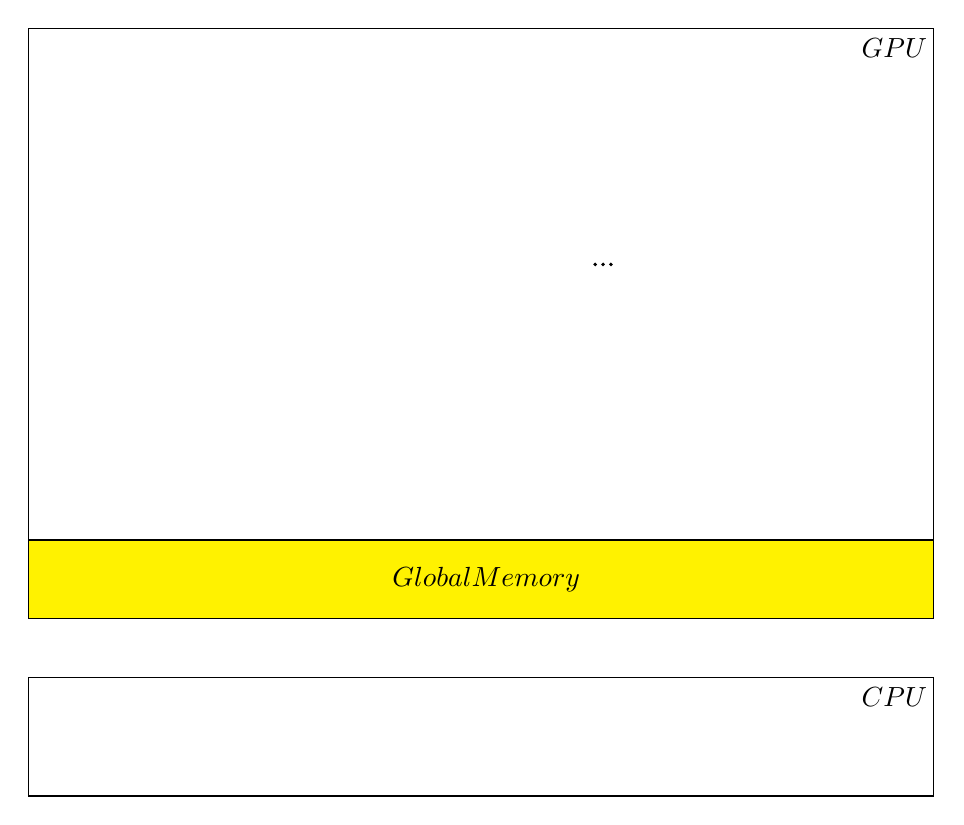
\begin{tikzpicture}
			
			\node[rectangle,
			draw = black,
			text = black,
			anchor = center,
			align=center,
			minimum width = 11.5cm, 
			minimum height = 7.5cm] (cpu1) at (3.75 cm, -0.75cm) {};
			\node[anchor=center] at (9 cm, 2.75 cm) {$GPU$};
			
			\node[rectangle,
			draw = black,
			text = black,
			anchor = center,
			align=center,
			minimum width = 11.5cm, 
			minimum height = 1.5cm] (cpu1) at (3.75 cm, -6cm) {};
			\node[anchor=center] at (9 cm, -5.5 cm) {$CPU$};
			
			
			\block{0}{0}{0}
			\block{3.2}{0}{1}
			\block{7.4}{0}{n}
			
			% Dots
			\node  at (5.2cm,0cm) [circle, fill, inner sep=0.5pt] {};
			\node  at (5.3cm,0cm) [circle, fill, inner sep=0.5pt] {};
			\node  at (5.4cm,0cm) [circle, fill, inner sep=0.5pt] {};
			
			
			\node[rectangle,
			draw = black,
			text = black,
			anchor = center,
			fill = yellow,
			align=center,
			minimum width = 11.5cm, 
			minimum height = 1cm] (cpu1) at (3.75 cm,-4cm) {};
			\node[anchor=west] at (2.5 cm, -4 cm) {$Global Memory$};
			
		\end{tikzpicture}
	\end{center}
\end{figure}

\subsubsection{Asynchronous Operations} \label{sec:async}

There are two types of engines that can be used to execute kernels in CUDA streams: copy engines and kernel engines. Copy engines are used to copy data between host and device memory, and between different types of memory on the device. Kernel engines are used to execute CUDA kernels. The number of individual engines depends on the actual hardware, lower end GPUs usually have a single kernel and a copy engine, more advanced architectures can have more than one copy or kernel engine.

A CUDA stream is a sequence of commands that are executed in order on a CUDA device. Streams can be used to improve the runtime of a CUDA program by overlapping the execution of different kernels. For example, a copy kernel can be executed in one stream while a compute kernel is executed in another stream. This overlap can lead to a significant performance improvement.


\subsubsection{Synchronization}

Whilst threads within a block can be synchronized, this is not the case for the blocks launched from a kernel. The only real synchronization technique, is to wait for a kernel, meaning all blocks associated with this kernel, to finish and execute a consecutive task using another kernel. 

Since the GPU is limited in its computing and also memory capabilities, the number of blocks which are run in parallel are limited, therefore CUDA cannot give us any guarantee, weather a set of blocks are run serially or in parallel. Some of the blocks might be run in parallel, meanwhile others are run serially. This very constraint, forces the programmer to rethink algorithms and think of ways, how individual subproblems can be run somewhat independently of each other. 

There exists however a way to communicate between blocks in a safe way. Atomic operations can be performed on global memory without any race conditions.
\begin{figure}
	\begin{center}
		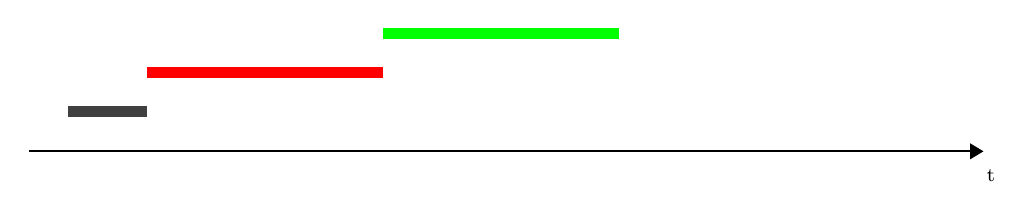
\begin{tikzpicture}
			% draw horizontal line   
			\draw[thick, -Triangle] (0,0) -- (\textwidth,0) node[font=\scriptsize,below left=3pt and -8pt]{t};
			\draw[darkgray, line width=4pt] 
			(0.5,.5) -- +(1,0);
			
			\draw[red, line width=4pt] 
			(1.5,1.0) -- +(3,0);
			
			\draw[green, line width=4pt] 
			(4.5,1.5) -- +(3,0);
	
		\end{tikzpicture}
	\end{center}
	\caption{timeline}
	\label{u}
\end{figure}

\subsection{Streams}

As described in section \ref{sec:async}, we can leverage streams to improve the runtime a CUDA accelerated application. The way we make use of streams is simple, each thread performs all its computations using on a unique stream. Since leveraging streams only improves the runtime in low numbers because the actual copy and kernel engines are not very numerous, this variant is very simple and effective. We have observed that using more streams on the individual threads does not improve the runtime, quiet contrary it can have a negative impact. 


\subsection{Memory Management}

We can use several strategies in order to improve the performance of memory allocation: 

\begin{enumerate}
	\item \textbf{Pinned Memory} As the GPU cannot access the default paged memory directly, when copying memory from the host to the device, the memory must first be copied to pinned memory. This means if we use pinned memory directly with $cudaMallocHost()$, data transfers can be around twice as fast. In our implementation we use pinned memory for all data, which need to be either sent from the host to device or vice versa.
	\item \textbf{Reuse Memory} We can avoid allocation and freeing commands altogether and instead reuse previously allocated memory whenever possible. In our implementation we allocate the memory in the very beginning, whereas we have a fixed number of particles and a fixed upper limit for the number of cells. This is true for both the CPU and GPU memory.
\end{enumerate}

\subsection{GPU Accelerated Count Left}


We have described a CPU implementation of the countLeftService. In this section we explain how we can port this problem to the GPU. In essence we can use a general reduction as a basis version, and adapt it to sum up up elements which fulfill a certain condition, where the condition is being smaller than a given value.

Optimized reductions in CUDA are well documented and explained by the NVIDIA developer team. We make use of a reduction introduced by \TODO{Reference} and adapt it slightly to fit our needs. We will reiterate over the important optimization aspects and finally point out the specific adaptations we have made. 

We split the array of particles which are contained within one cell into smaller slices, where each slice fits one block. Then the subproblems or blocks can be run independently from each other, in other words individual blocks can be executed in parallel or also serially without any conflicts or need for block level synchronization. After running the conditional summation on each slice of the array, we end up with a an array of results. These results can then be summed together on CPU using a simple iterator. Alternatively we could invoke another sum reduction kernel for this task.


\subsubsection{Schedule}

The entire schedule of the ORB is depicted in figure \ref{fig:orbgpup}. In a first step we call the initialize service, where the necessary data is allocated on all devices and the particles are loaded. Furthermore the initial SPTDS is constructed, which essentially only consists of the root node, encompassing the entire domain and all the particles. Next we enter the main loop of ORB, it iterates until it has constructed a SPTDS with the desired size. Within the loop the count service is called, computing the number of cells for each cell summed over all the threads in the system. To prepare the data for the GPU transfer we make the temporary array using the make axis service, which is then sent to the GPU. 
We can now start with the root finding process, where we count the particles left of the initial cut position using the Count Left Service. Depending on the outcome, we then improve the cut position and repeat until a nearly perfect cut is found for all the leaf cells of the current SPTDS. We now generate two new child cells using the computed cut positions for all leaf cells of the current SPTDS and enrich the current SPTDS with the newly generated cells. Finally the particles array is partitioned accordingly. 
The tree building loop is then repeated or if the desired size of the SPTDS is reached, we exit the loop and call the finalize service to free the allocated memory.


\begin{figure}[H]
	\begin{center}
		\begin{tikzpicture}
			
			\timeline{6}{14}{3}
			
			
			\parallelloop{-2}{12.5}{8}{1.5}{loop till tree built};
			
			\parallelloop{-1}{9.5}{7}{5.5}{loop till cut found};
			
			\communication{Init}{0}{7}{13};
			
			\communication{Count}{0}{7}{12};
			
			\communication{Make Axis}{0}{7}{11};
			
			\communication{Copy Particles To GPU}{0}{7}{10};
			
			\communication{Count Left GPU}{0}{7}{9};
			
			\process{improve \\ cut}{0}{8};
			
			
			\process{generate\\ new \\ cells}{0}{5};
						
			\communication{Partition}{0}{7}{2};
			
			\communication{Finalize}{0}{7}{1};
			
			
		\end{tikzpicture}
	\end{center}
	\caption{Parallelized ORB GPU version}
	\label{fig:orbgpup}
\end{figure}

\subsubsection{Service}

The Count Left Service invokes the Count Left kernel exactly once for every leaf cell of the current SPTDS. Meaning on level 0 of the tree there is only one kernel per thread being executed, when proceeding to further levels, the number of kernels is equivalent to $2^{level}$. 
The number of blocks can be determined by the number of particles in this cell $n_{cell}$ divided by the number of threads per block which is set to 256 and finally we divide this further by the number of elements per thread $r$. 

Since we can pass all the relevant information regarding a cell as input parameters to the cell, there is no need to copy any additional data from the CPU to the GPU. We only need to copy back the results from the GPU to the GPU.

\subsubsection{Kernel Code}\label{sec:countleftcode}
The actual kernel code is depicted in figure \ref{cuda:reduction}. The input parameters of the reduction kernel (line 13-16), the input data, which is in sequential order the particles, the output array, which is the results of the kernel, the cut position and finally the total number of elements contained within the cell. 
We will 
\begin{itemize}
	\item \textbf{Leverage Shared Memory} 
	In the code on line 17 we invocate the shared memory, where is equivalent to the block size, which corresponds to a single float per thread. In a next step (lines 24-27) we apply our condition and copy the results to shared memory. This allows us to work exclusively with shared memory, reducing the amount of costly accesses performed on global memory.
	
	\item \textbf{Increase Thread Occupancy} There exists an optimum when considering the number of operation performed by a single thread. In order to adapt the number of ops dynamically, we iterate over a certain number of elements in the global memory, as seen in lines 24-27. The input parameter n defines the total number of particles. Therefore if we reduce the total number of blocks by a factor of $r$, the while loop will iterate over $r$ elements. In our case we set $r$ to 32. \TODO{Say why optimal value}
	
	\item \textbf{Meta Programming} The reduction is optimized by using a template, which indicates the total number of thread per block, which is equivalent to the blockSize. Since the template is evaluated at compile time, all the if statements taking blockSize as a parameter in figure do not cause any performance loss. In fact, because we are able to unroll loops, which would be evaluated at runtime, we increase the performance of the code. 
	
	\item \textbf{Avoiding Warp Divergence} Each time we we have an control statement in the code, we introduce a divergence. On the GPU these divergences become especially bad when they are introduced inside a warp. This means that any of the threads of the 32 threads in a warp, have to execute a different code than the rest. For this reason, the $warpReduce$ method as on line 2-9 is introduced. We can see on line 32 in figure \ref{cuda:reduction} that this method is only executed when we reach 32 elements in the shared memory, which remain to be added together. Inside the warp reduce method, we again encounter an unrolled loop, but in this case we have no if statements that could generate a divergence. The if statements which are present, are as mentioned, evaluated at compile time only. Inside a warp we are also not dependent on synchronization, thus the thread synchronization call can be omitted as well. Note that this implementation will perform many unnecessary operations, but this does not affect the performance negatively.
	
\end{itemize}


\begin{comment}
\newcommand{\kernel}[3]{
\foreach \i in {1,...,#3}
{
	\draw[darkgray, line width=4pt] 
	({#1 cm / #3 cm * (\i-1 cm)  - 0.2 cm * (\i-1 cm)} ,#2 cm) -- 
	+({(#1 cm / #3 cm)  - 0.2 cm}, 0cm);
	
}
}
	
\begin{figure}
	\begin{center}
		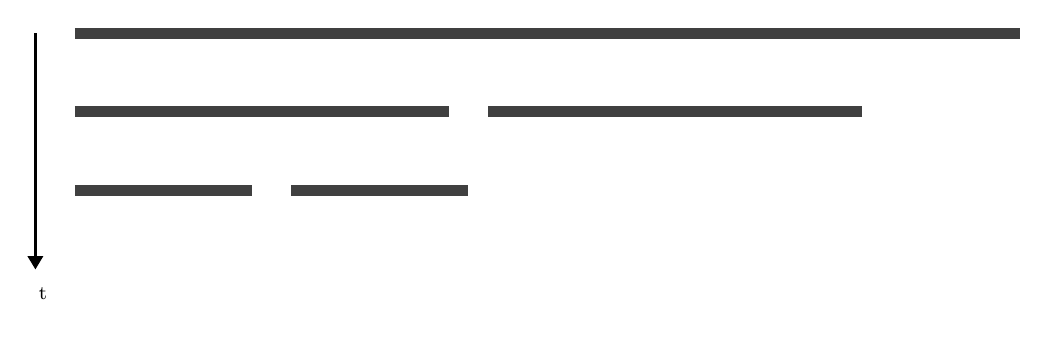
\begin{tikzpicture}
			% draw horizontal line   
			\kernel{10}{4}{4};
			
			\draw[thick, -Triangle] (-0.5cm,0cm) -- (-.5cm,-3cm) node[font=\scriptsize,below left=3pt and -8pt]{t};
			
			% l1
			\draw[darkgray, line width=4pt] 
			(0,0) -- +(12,0);
			
			% l2
			\draw[darkgray, line width=4pt] 
			(0cm,-1cm) -- +(4.75cm,0);
			
			\draw[darkgray, line width=4pt] 
			(5.25cm,-1cm) -- +(4.75cm,0);
			
			
			\draw[darkgray, line width=4pt] 
			(0cm,-2cm) -- +(2.25cm,0);
			
			\draw[darkgray, line width=4pt] 
			(2.75cm,-2cm) -- +(2.25cm,0);


			
		\end{tikzpicture}
	\end{center}
	\caption{timeline}
	\label{u}
\end{figure}
\end{comment}

\begin{figure}[H]
	\begin{lstlisting}[language=c++]
template <unsigned int blockSize>
extern __device__ void warpReduce(volatile int *sdata, unsigned int tid) {
	if (blockSize >= 64) sdata[tid] += sdata[tid + 32];
	if (blockSize >= 32) sdata[tid] += sdata[tid + 16];
	if (blockSize >= 16) sdata[tid] += sdata[tid + 8];
	if (blockSize >= 8) sdata[tid] += sdata[tid + 4];
	if (blockSize >= 4) sdata[tid] += sdata[tid + 2];
	if (blockSize >= 2) sdata[tid] += sdata[tid + 1];
}

template <unsigned int blockSize>
extern __global__ void reduce(
	float *g_idata,
	 unsigned int*g_odata, 
	 float cut, 
	 int n) {
	__shared__ int sdata[blockSize];
	
	unsigned int tid = threadIdx.x;
	unsigned int i = blockIdx.x*(blockSize) + threadIdx.x;
	unsigned int gridSize = blockSize*gridDim.x;
	sdata[tid] = 0;
	
	while (i < n) {
		sdata[tid] += (g_idata[i] <= cut);
		i += gridSize;
	}
	__syncthreads();
	
	if (blockSize >= 512) {
		if (tid < 256) {
			sdata[tid] += sdata[tid + 256];
		}
		__syncthreads();
	}
	if (blockSize >= 256) {
		if (tid < 128) {
			sdata[tid] += sdata[tid + 128];
		} __syncthreads();
	}
	if (blockSize >= 128) {
		if (tid < 64) {
			sdata[tid] += sdata[tid + 64];
		} __syncthreads();
	}
	if (tid < 32) {
		warpReduce<blockSize>(sdata, tid);
	}
	if (tid == 0) {
		g_odata[blockIdx.x] = sdata[0];
	}
}
	\end{lstlisting}
	\caption{Reduction in CUDA}
	\label{cuda:reduction}
\end{figure}


We execute the reduction kernel once for each cell, where we distribute the particles within the cell among a set of blocks. This makes the implementation straight forward but as we increase the number of cells, we make make more calls to the reduction kernel. This is problematic because each initialization of a kernel comes with some overhead, degrading the performance gradually with the tree traversal, as the overhead to computation ratio becomes more and more unfavorable.  



\subsection{Improved GPU Accelerated Count Left}

To solve the degrading performance problem we make some changes to the kernel and the overall schedule. The main idea is to prepare all the necessary data for each of the blocks, meaning each block knows which slice of the particles data is has to iterate over and the cut position which was chosen for the cell owning the range of particles. 
We will explain the improved version using an example: Let us consider $cell_2$ with a volume that encompasses particles in the range 0 - 6144. $cell_3$ encompasses particles in the range 6144 - 12288. Considering a blocksize of 256 threads and a number of elements per thread of 16, each block processes $256 * 16 = 4096$ elements. In this case we reserve two blocks for each cell, where the first block processes elements 0 - 4096, the second one 4096 - 6144, the third 6144 - 10240 and finally the last block processes 10240 - 12288. This ensures that each block only iterates over the particles owned by a single cell, and no further control statements are necessary inside the kernel. There might be some kernels with a very low workload, in the worst case a kernel only processes a single element, but in the average case the performance penalty is minor. We observe a slight reduction in performance and cl	

\subsubsection{Schedule}

\begin{figure}[H]
	\begin{center}
		\begin{tikzpicture}
			
			\timeline{6}{15}{3}
			
			
			\parallelloop{-2}{13.5}{8}{1.5}{loop till tree built};
			
			\parallelloop{-1}{9.5}{7}{5.5}{loop till cut found};
			
			\communication{Init}{0}{7}{14};
			
			\communication{Count}{0}{7}{13};
			
			\communication{Make Axis}{0}{7}{12};
			
			\communication{Copy Particles To GPU}{0}{7}{11};
			
			\communication{Copy Cells To GPU}{0}{7}{10};
			
			\communication{Count Left GPU}{0}{7}{9};
			
			\process{improve \\ cut}{0}{8};
			
			
			\communication{Partition}{0}{7}{5};
			
			\communication{Finalize}{0}{7}{1};
			
			\process{generate\\ new \\ cells}{0}{4};
			
		\end{tikzpicture}
	\end{center}
	\caption{Parallelized ORB GPU version 2}
	\label{fig:orbgpup2}
\end{figure}


\subsubsection{Code}

\begin{figure}[H]
	\begin{lstlisting}[language=c++]
template <unsigned int blockSize>
extern __global__ void reduce(
float * g_idata,
unsigned int * g_begins,
unsigned int * g_ends,
float * g_cuts,
unsigned int * a_index,
unsigned int * g_odata) {
	
	__shared__ unsigned int s_data[blockSize];
	__shared__ unsigned int s_index;
	
	unsigned int tid = threadIdx.x;
	
	if (tid == 0) {
		s_index = atomicAdd(a_index, 1);
	}
	__syncthreads();
	
	const unsigned int begin = g_begins[s_index];
	const unsigned int end = g_ends[s_index];
	const float cut = g_cuts[s_index];
	
	unsigned int i = begin + tid;
	//const unsigned int gridSize = blockSize*gridDim.x;
	s_data[tid] = 0;
	
	while (i < end) {
		s_data[tid] += (g_idata[i] <= cut);
		i += blockSize;
	}
	__syncthreads();
	
	if (blockSize >= 512) {
		if (tid < 256) {
			s_data[tid] += s_data[tid + 256];
		}
		__syncthreads();
	}
	if (blockSize >= 256) {
		if (tid < 128) {
			s_data[tid] += s_data[tid + 128];
		} __syncthreads();
	}
	if (blockSize >= 128) {
		if (tid < 64) {
			s_data[tid] += s_data[tid + 64];
		} __syncthreads();
	}
	if (tid < 32) {
		warpReduce<blockSize>(s_data, tid);
	}
	if (tid == 0) {
		g_odata[s_index] = s_data[0];
	}
}
	\end{lstlisting}
	\caption{Reduction in CUDA}
	\label{cuda:reduction2}
\end{figure}

\subsection{GPU Accelerated Partitioning}

The main bottlenecks of the orb algorithm are now the data transfer between the CPU and GPU and the partitioning of the data. Both problems can be resolved by partitioning the array on the GPU directly thus also removing the need to transfer the data back and forth between the CPU and the GPU.

We describe measurements which were done using the reduction in CUDA, we mention how the reduction cannot necessarily be improved a lot and that the data transfer between the GPU and CPU is the main bottleneck now. We mention how building the tree on the does not make a lot of sense. We explain why instead we focus our efforts to implement a GPU reshuffling method, which can improve runtime by reducing the reshuffling costs and also remove CPU GPU transfers between invocations of the binary cut algorithm altogether. 

\subsubsection{Schedule}

\begin{figure}[H]
	\begin{center}
		\begin{tikzpicture}
			
			\timeline{6}{14}{3}
			
			
			\parallelloop{-2}{11.5}{8}{1.5}{loop till tree built};
			
			\parallelloop{-1}{9.5}{7}{5.5}{loop till cut found};
			
			\communication{Init}{0}{7}{13};
			
			\communication{Copy Particles To GPU}{0}{7}{12};
			
			\communication{Count}{0}{7}{11};
		
			
			\communication{Copy Cells To GPU}{0}{7}{10};
			
			\communication{Count Left GPU}{0}{7}{9};
			
			\process{improve \\ cut}{0}{8};
			
			
			\communication{Partition}{0}{7}{5};
			
			\communication{Finalize}{0}{7}{1};
			
			\process{generate\\ new \\ cells}{0}{4};
			
		\end{tikzpicture}
	\end{center}
	\caption{Parallelized ORB with GPU counting and GPU partitioning}
	\label{fig:orbgpup3}
\end{figure}

We add a timeline which is based on measurements with a CUDA enhanced binary cut algorithm. 


\begin{figure}[H]
	\begin{center}
		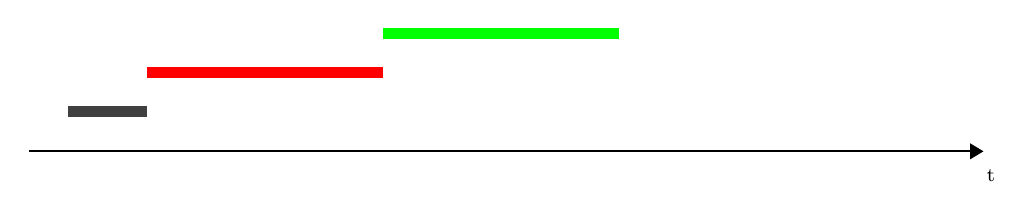
\begin{tikzpicture}
			% draw horizontal line   
			\draw[thick, -Triangle] (0,0) -- (\textwidth,0) node[font=\scriptsize,below left=3pt and -8pt]{t};
			\draw[darkgray, line width=4pt] 
			(0.5,.5) -- +(1,0);
			
			\draw[red, line width=4pt] 
			(1.5,1.0) -- +(3,0);
			
			\draw[green, line width=4pt] 
			(4.5,1.5) -- +(3,0);
			
		\end{tikzpicture}
	\end{center}
	\caption{timeline}
	\label{u}
\end{figure}

The partitioning algorithm is a widely used concept and there are various implementations used in different variants of the quick-sort algorithm. The overall design of the implementation is guided by \TODO{Insert ref} and the scan is taken from GPU Gems \TODO{Insert ref}. The main and probably only disadvantage of partitioning the particle array on the GPU, is that it cannot be done in place, thus we need another temporary array allocated on the GPU memory which further restricts the total number of particles. Furthermore we need to store the permutations, because we need to apply them to the other axes as well. We could as well simply perform all permutations from the same kernel at the same time, but this would require 3 temporary arrays, thus reducing the total number of particles by a factor of 2. The solution with the partition array and a single temporary array only results in a reduction of the particles by a factor of $\frac{5}{3}$. 	

\begin{itemize}
	\item As we increase the number of cells, we make more calls to the reduction kernel 
	
\end{itemize}

\subsubsection{Code}

\begin{figure}[H]
	
\begin{lstlisting}[language=c++]
template <unsigned int blockSize>
__global__ void partition(
unsigned int * g_offsetLessEquals,
unsigned int * g_offsetGreater,
float * g_idata,
float * g_odata,
unsigned int * g_permutations,
float pivot,
unsigned int nLeft,
unsigned int n) {
	__shared__ unsigned int s_lessEquals[blockSize * 2];
	__shared__ unsigned int s_greater[blockSize * 2];
	__shared__ unsigned int s_offsetLessEquals;
	__shared__ unsigned int s_offsetGreater;
	
	unsigned int tid = threadIdx.x;
	
	unsigned int i = blockIdx.x * blockSize * 2 + 2 * tid;
	unsigned int j = blockIdx.x * blockSize * 2 + 2 * tid + 1;
	
	bool f1, f2, f3, f4;
	if (i < n) {
		f1 = g_idata[i] <= pivot; f2 = not f1;
		s_lessEquals[2*tid] = f1;
		s_greater[2*tid] = f2;
	} else {
		f1 = false; f2 = false;
		s_lessEquals[2*tid] = 0;
		s_greater[2*tid] = 0;
	}
	
	if (j < n) {
		f3 = g_idata[j] <= pivot; f4 = not f3;
		s_lessEquals[2*tid+1] = f3;
		s_greater[2*tid+1] = f4;
	} else {
		f3 = false; f4 = false;
		s_lessEquals[2*tid+1] = 0;
		s_greater[2*tid+1] = 0;
	}
	
	__syncthreads();
	
	scan(s_lessEquals, tid, blockSize * 2 );
	scan(s_greater, tid, blockSize * 2);
	\end{lstlisting}
	\caption{Partitioning kernel I}
	\label{cuda:partitionI}
\end{figure}



\begin{figure}
\begin{lstlisting}[language=c++]
	
	__syncthreads();
	
	if (tid == blockSize - 1) {
		s_offsetLessEquals = 
		atomicAdd(g_offsetLessEquals, s_lessEquals[blockSize*2-1] + f3);
		s_offsetGreater = 
		atomicAdd(g_offsetGreater, s_greater[blockSize*2-1] + f4);
	}
	
	__syncthreads();
	
	unsigned int indexA = (s_lessEquals[2*tid] + s_offsetLessEquals) * f1 +
	(s_greater[2*tid] + s_offsetGreater + nLeft) * f2;
	
	unsigned int indexB = (s_lessEquals[2*tid+1] + s_offsetLessEquals) * f3 +
	(s_greater[2*tid+1] + s_offsetGreater + nLeft) * f4;
	
	if (i < n) {
		g_odata[indexA] = g_idata[i];
		g_permutations[i] = indexA;
	}
	
	if (j < n) {
		g_odata[indexB] = g_idata[j];
		g_permutations[j] = indexB;
	}
}
	\end{lstlisting}
	\caption{Partitioning kernel II}
	\label{cuda:partitionII]}
\end{figure}


\begin{figure}[H]
	\begin{lstlisting}[language=c++]
__device__ void scan(volatile unsigned int * s_idata, unsigned int thid, unsigned int n) {
	unsigned int offset = 1;
	for (unsigned int d = n>>1; d > 0; d >>= 1) // build sum in place up the tree
	{
		__syncthreads();
		if (thid < d)
		{
			unsigned int ai = offset*(2*thid+1)-1;
			unsigned int bi = offset*(2*thid+2)-1;
			s_idata[bi] += s_idata[ai];
		}
		offset *= 2;
	}
	if (thid == 0) { s_idata[n - 1] = 0; } // clear the last element
	for (unsigned int d = 1; d < n; d *= 2) // traverse down tree & build scan
	{
		offset >>= 1;
		__syncthreads();
		if (thid < d)
		{
			unsigned int ai = offset*(2*thid+1)-1;
			unsigned int bi = offset*(2*thid+2)-1;
			unsigned int t = s_idata[ai];
			s_idata[ai] = s_idata[bi];
			s_idata[bi] += t;
		}
	}
}
	\end{lstlisting}
	\caption{Device Scan Kernel}
	\label{cuda:scan}
\end{figure}



\begin{figure}[H]
	\begin{lstlisting}[language=c++]
template <unsigned int blockSize>
__global__ void permute(
float * g_idata,
float * g_odata,
unsigned int * g_permutations,
int n) {
	unsigned int tid = threadIdx.x;
	
	unsigned int i = blockIdx.x * blockSize * 2 + 2 * tid;
	unsigned int j = blockIdx.x * blockSize * 2 + 2 * tid + 1;
	//unsigned int gridSize = blockSize*2*gridDim.x;
	
	if (i < n) {
		g_odata[g_permutations[i]] = g_idata[i];
	}
	
	if (j < n) {
		g_odata[g_permutations[j]] = g_idata[j];
	}
}
	\end{lstlisting}
	\caption{Device Permute Kernel}
	\label{cuda:permute}
\end{figure}



\subsection{Integration into PKDGRAV}



\newpage
\section{Performance Analysis of ORB}

We will use two system for our performance analysis. One is the Summit supercomputer which has been described in section 3.1. The other has the following specs:


AMD EPYC 7702 64-Core Processor, Tesla T4.


\subsection{Methodology}

\subsection{Results}


\begin{comment}
	\begin{figure}[H]
		\begin{center}
			\begin{tikzpicture}
				\begin{axis}[
					height=10cm,width=13cm, 
					title={Measured Performance with $d = 1024$},
					xlabel={Particle Count},
					ylabel={Execution Time (ms)},
					]
					
					\foreach \i in {0,...,3}{
						\pgfmathsetmacro\suffix{int(pow(2,\i))};
						
						\addplot +[] 
						table [col sep=comma, x=N, y=time] 
						{../../code/out/measurements\suffix.csv};
						
						\addlegendentryexpanded{\# $\suffix$};
						
					}	
				\end{axis}
			\end{tikzpicture}
		\end{center}
	\end{figure}
\end{comment}


\subsection{Comparison to Theoretical Model}


\subsection{Conclusion}


% Use for reduction explanation https://texample.net/tikz/examples/database-decimation-process/
\bibliographystyle{unsrt}
\bibliography{reference}

\end{document}
